
\section{Related Work on Post-Training Quantization}

Post-training quantization has received considerable attention for large language models, where memory bandwidth is the dominant deployment cost and reducing bit-width directly lowers that cost without retraining. The discussion here is restricted to post-training methods — those that determine the quantized representation under limited post-training resources, without an additional training or fine-tuning phase. Quantization-aware training operates in a fundamentally different regime: it requires simulating quantization throughout a training or fine-tuning process, and its computational cost makes it unsuitable for LLMs at scale. OmniQuant notes that many LLM quantization methods specifically prioritize training-free PTQ for this reason \cite{shao2023omniquant}. Computationally efficient QAT variants still report 41 hours on a single A100-80GB for a 2-bit LLaMA-2-70B run \cite{tang2024efficientqat}, and standard QAT for 7B models requires more than 70GB of GPU memory \cite{bondarenko2024lrqat}. LLM-QAT makes the distinction concrete: quantization-aware training for LLMs is not a quantization formula but a full data-free distillation procedure over the pretrained model \cite{liu2023llm}, placing it in the same regime as recovery-based compression rather than post-training compression.

The methods reviewed here differ in how they control quantization error within the PTQ setting. The related work is organized by the dominant mechanism: rotation-based methods that redistribute activation energy before discretization, salience-based methods that identify and protect sensitive weights or channels, compensation-based methods that use second-order curvature to correct for quantization decisions locally, and optimization-based methods that tune quantization parameters directly on calibration data.

\subsection{Problem Setting and Taxonomy}

Post-train quantization (PTQ) reduces numerical precision after the full-precision phase. Conversion to lower bit-widths such as INT4 and INT8 lowers memory traffic and permits efficient integer arithmetic during inference. This makes PTQ particularly important for large language models, where deployment cost is often dominated by memory movement rather than arithmetic alone. Accuracy preservation, however, remains difficult. Moderate regimes typically focus on controlling layer-wise reconstruction error, whereas extreme regimes at $2$--$3$ bits must additionally address severe sensitivity to activation outliers and discrete approximation error \cite{frantar2022gptq,chee2024quip,ashkboos2024quarot}.

\begin{figure}[H]
  \centering
  \makebox[\textwidth][c]{%
    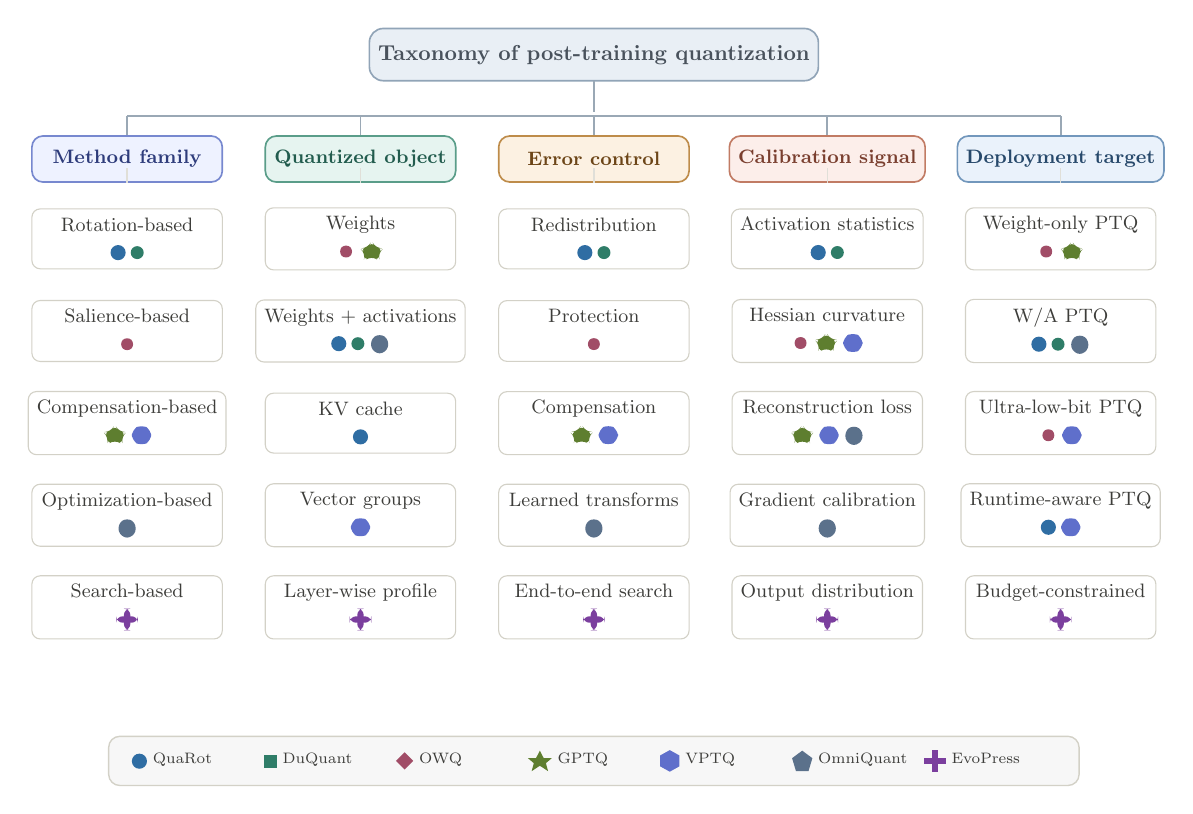
\begin{tikzpicture}[
  every node/.style={inner sep=4pt},
  font=\sffamily,
  scale=0.78,
  transform shape
]

\definecolor{rootbg}   {HTML}{E9EFF5}
\definecolor{rootbdr}  {HTML}{91A4B7}
\definecolor{trunkclr} {HTML}{9AA8B5}
\definecolor{leafbdr}  {HTML}{D3D1C7}
\definecolor{leaftxt}  {HTML}{3D3D3A}

\definecolor{ax1bg}  {HTML}{EEF2FF} \definecolor{ax1bd}  {HTML}{7788CF} \definecolor{ax1tx}  {HTML}{2E3C7B}
\definecolor{ax2bg}  {HTML}{E6F4F0} \definecolor{ax2bd}  {HTML}{5A9D89} \definecolor{ax2tx}  {HTML}{225C4E}
\definecolor{ax3bg}  {HTML}{FCF1E2} \definecolor{ax3bd}  {HTML}{BE8C4A} \definecolor{ax3tx}  {HTML}{6C4517}
\definecolor{ax4bg}  {HTML}{FCEEEA} \definecolor{ax4bd}  {HTML}{C17B64} \definecolor{ax4tx}  {HTML}{7A3F2F}
\definecolor{ax5bg}  {HTML}{EAF2FB} \definecolor{ax5bd}  {HTML}{7297BC} \definecolor{ax5tx}  {HTML}{27496B}

\definecolor{cquarot}  {HTML}{2F6DA3}
\definecolor{cduquant} {HTML}{2F7D68}
\definecolor{cowq}     {HTML}{A14D67}
\definecolor{cgptq}    {HTML}{5E7E2F}
\definecolor{cvptq}    {HTML}{5F6FCB}
\definecolor{comni}    {HTML}{5B718B}
\definecolor{cevopress}{HTML}{7B3F9E}

\newcommand{\symQuaRot}{\tikz[baseline=-1pt]\fill[cquarot] (0,0) circle (3.5pt);}
\newcommand{\symDuQuant}{\tikz[baseline=-1pt]\fill[cduquant] (-3pt,-3pt) rectangle (3pt,3pt);}
\newcommand{\symOWQ}{\tikz[baseline=-1pt]\fill[cowq] (0,4pt) -- (4pt,0) -- (0,-4pt) -- (-4pt,0) -- cycle;}
\newcommand{\symGPTQ}{\tikz[baseline=-1pt]
  \fill[cgptq] (0,5pt) -- (1.8pt,1.5pt) -- (5.5pt,1.5pt) -- (2.8pt,-0.8pt)
              -- (3.8pt,-4.5pt) -- (0,-2pt) -- (-3.8pt,-4.5pt)
              -- (-2.8pt,-0.8pt) -- (-5.5pt,1.5pt) -- (-1.8pt,1.5pt) -- cycle;}
\newcommand{\symVPTQ}{\tikz[baseline=-1pt]
  \fill[cvptq] (0,5pt) -- (4.5pt,2.5pt) -- (4.5pt,-2.5pt)
              -- (0,-5pt) -- (-4.5pt,-2.5pt) -- (-4.5pt,2.5pt) -- cycle;}
\newcommand{\symOmni}{\tikz[baseline=-1pt]
  \fill[comni] (0,5pt) -- (4.7pt,1.5pt) -- (2.9pt,-4.5pt)
              -- (-2.9pt,-4.5pt) -- (-4.7pt,1.5pt) -- cycle;}
\newcommand{\symEvoPress}{\tikz[baseline=-1pt]{
  \fill[cevopress] (-1.5pt,-5pt) rectangle (1.5pt,5pt);
  \fill[cevopress] (-5pt,-1.5pt) rectangle (5pt,1.5pt);}}

\def\rootY{0}
\def\trunkY{-1.0}
\def\headerY{-1.7}
\def\firstY{-3.0}
\def\rowstep{-1.50}

\def\xI{0}
\def\xII{3.8}
\def\xIII{7.6}
\def\xIV{11.4}
\def\xV{15.2}

\node[draw=rootbdr, fill=rootbg, rounded corners=5pt,
      minimum width=7.2cm, minimum height=0.85cm,
      font=\normalsize\bfseries\color{rootbdr!50!black},
      line width=0.6pt] at (7.6,\rootY) (ROOT) {Taxonomy of post-training quantization};

\draw[trunkclr, line width=0.7pt] (ROOT.south) -- ++(0,-0.5);
\draw[trunkclr, line width=0.7pt] (\xI,\trunkY) -- (\xV,\trunkY);
\foreach \cx in {\xI,\xII,\xIII,\xIV,\xV} {
  \draw[trunkclr, line width=0.7pt] (\cx,\trunkY) -- (\cx,\headerY+0.375);
}
\draw[trunkclr, line width=0.7pt] (7.6,\trunkY-0.5) -- (7.6,\trunkY);

% ---- Column 1: Method family ----
\node[draw=ax1bd, fill=ax1bg, rounded corners=4pt,
      minimum width=3.1cm, minimum height=0.75cm,
      font=\small\bfseries\color{ax1tx}, align=center,
      line width=0.6pt] at (\xI,\headerY) (H1) {Method family};
\draw[leafbdr!70, line width=0.5pt] (H1.south) -- ++(0, 5*\rowstep + 0.5cm);
\foreach[count=\i] \txt/\sym in {
  {Rotation-based}/{\symQuaRot\;\symDuQuant},
  {Salience-based}/{\symOWQ},
  {Compensation-based}/{\symGPTQ\;\symVPTQ},
  {Optimization-based}/{\symOmni},
  {Search-based}/{\symEvoPress}
}{
  \pgfmathsetmacro\ypos{\firstY + (\i-1)*\rowstep}
  \node[draw=leafbdr, fill=white, rounded corners=3pt,
        minimum width=3.1cm, minimum height=0.85cm,
        font=\small\color{leaftxt}, align=center,
        line width=0.4pt] at (\xI,\ypos) {\txt\\\footnotesize\sym};
}

% ---- Column 2: Quantized object ----
\node[draw=ax2bd, fill=ax2bg, rounded corners=4pt,
      minimum width=3.1cm, minimum height=0.75cm,
      font=\small\bfseries\color{ax2tx}, align=center,
      line width=0.6pt] at (\xII,\headerY) (H2) {Quantized object};
\draw[leafbdr!70, line width=0.5pt] (H2.south) -- ++(0, 5*\rowstep + 0.5cm);
\foreach[count=\i] \txt/\sym in {
  Weights/{\symOWQ\;\symGPTQ},
  {Weights + activations}/{\symQuaRot\;\symDuQuant\;\symOmni},
  {KV cache}/{\symQuaRot},
  {Vector groups}/{\symVPTQ},
  {Layer-wise profile}/{\symEvoPress}
}{
  \pgfmathsetmacro\ypos{\firstY + (\i-1)*\rowstep}
  \node[draw=leafbdr, fill=white, rounded corners=3pt,
        minimum width=3.1cm, minimum height=0.85cm,
        font=\small\color{leaftxt}, align=center,
        line width=0.4pt] at (\xII,\ypos) {\txt\\\footnotesize\sym};
}

% ---- Column 3: Error control ----
\node[draw=ax3bd, fill=ax3bg, rounded corners=4pt,
      minimum width=3.1cm, minimum height=0.75cm,
      font=\small\bfseries\color{ax3tx}, align=center,
      line width=0.6pt] at (\xIII,\headerY) (H3) {Error control};
\draw[leafbdr!70, line width=0.5pt] (H3.south) -- ++(0, 5*\rowstep + 0.5cm);
\foreach[count=\i] \txt/\sym in {
  Redistribution/{\symQuaRot\;\symDuQuant},
  Protection/{\symOWQ},
  Compensation/{\symGPTQ\;\symVPTQ},
  {Learned transforms}/{\symOmni},
  {End-to-end search}/{\symEvoPress}
}{
  \pgfmathsetmacro\ypos{\firstY + (\i-1)*\rowstep}
  \node[draw=leafbdr, fill=white, rounded corners=3pt,
        minimum width=3.1cm, minimum height=0.85cm,
        font=\small\color{leaftxt}, align=center,
        line width=0.4pt] at (\xIII,\ypos) {\txt\\\footnotesize\sym};
}

% ---- Column 4: Calibration signal ----
\node[draw=ax4bd, fill=ax4bg, rounded corners=4pt,
      minimum width=3.1cm, minimum height=0.75cm,
      font=\small\bfseries\color{ax4tx}, align=center,
      line width=0.6pt] at (\xIV,\headerY) (H4) {Calibration signal};
\draw[leafbdr!70, line width=0.5pt] (H4.south) -- ++(0, 5*\rowstep + 0.5cm);
\foreach[count=\i] \txt/\sym in {
  {Activation statistics}/{\symQuaRot\;\symDuQuant},
  {Hessian curvature}/{\symOWQ\;\symGPTQ\;\symVPTQ},
  {Reconstruction loss}/{\symGPTQ\;\symVPTQ\;\symOmni},
  {Gradient calibration}/{\symOmni},
  {Output distribution}/{\symEvoPress}
}{
  \pgfmathsetmacro\ypos{\firstY + (\i-1)*\rowstep}
  \node[draw=leafbdr, fill=white, rounded corners=3pt,
        minimum width=3.1cm, minimum height=0.85cm,
        font=\small\color{leaftxt}, align=center,
        line width=0.4pt] at (\xIV,\ypos) {\txt\\\footnotesize\sym};
}

% ---- Column 5: Deployment target ----
\node[draw=ax5bd, fill=ax5bg, rounded corners=4pt,
      minimum width=3.1cm, minimum height=0.75cm,
      font=\small\bfseries\color{ax5tx}, align=center,
      line width=0.6pt] at (\xV,\headerY) (H5) {Deployment target};
\draw[leafbdr!70, line width=0.5pt] (H5.south) -- ++(0, 5*\rowstep + 0.5cm);
\foreach[count=\i] \txt/\sym in {
  {Weight-only PTQ}/{\symOWQ\;\symGPTQ},
  {W/A PTQ}/{\symQuaRot\;\symDuQuant\;\symOmni},
  {Ultra-low-bit PTQ}/{\symOWQ\;\symVPTQ},
  {Runtime-aware PTQ}/{\symQuaRot\;\symVPTQ},
  {Budget-constrained}/{\symEvoPress}
}{
  \pgfmathsetmacro\ypos{\firstY + (\i-1)*\rowstep}
  \node[draw=leafbdr, fill=white, rounded corners=3pt,
        minimum width=3.1cm, minimum height=0.85cm,
        font=\small\color{leaftxt}, align=center,
        line width=0.4pt] at (\xV,\ypos) {\txt\\\footnotesize\sym};
}

% ---- Legend ----
\def\legY{-11.5}
\def\legXstart{0.0}
\def\legstep{2.15}

\draw[leafbdr, fill=white!97!black, rounded corners=4pt, line width=0.5pt]
  (-0.3,\legY-0.4) rectangle (15.5,\legY+0.4);

\foreach[count=\k] \sym/\lbl in {
  \symQuaRot/QuaRot,
  \symDuQuant/DuQuant,
  \symOWQ/OWQ,
  \symGPTQ/GPTQ,
  \symVPTQ/VPTQ,
  \symOmni/OmniQuant,
  \symEvoPress/EvoPress
}{
  \pgfmathsetmacro\lx{\legXstart + (\k-1)*\legstep}
  \node[font=\scriptsize\color{leaftxt}, anchor=west, inner sep=2pt]
    at (\lx,\legY) {\sym~\lbl};
}

\end{tikzpicture}
%
  }
  \caption[Taxonomy of post-training quantization methods]{Taxonomy of post-training quantization methods. Rotation-based methods redistribute outliers, salience-based methods protect sensitive weights, compensation-based methods use curvature-guided correction, and optimization-based methods learn quantization parameters on calibration data.}
  \label{fig:type_of_ptq}
\end{figure}

Within this design space, a single chronological account is less informative than a taxonomy that separates the principal numerical and deployment choices underlying PTQ methods.

The method family constitutes the primary axis of the taxonomy, identifying the dominant mechanism for controlling quantization error. The remaining axes, by contrast, delineate the objects of quantization, the calibration information employed, and the deployment objective being prioritized. This analytical separation is essential, because post-training quantization methods that nominally target the same bit width can rest on substantially different numerical and system-level assumptions \cite{frantar2022gptq,lin2024awq,shao2023omniquant}.

Method family is the primary taxonomy axis, grouping techniques by their dominant error-control principle. Rotation-based methods redistribute activation energy before discretization. Salience-based methods protect statistically sensitive weights or channels. Compensation-based methods model interactions between local quantization decisions and the remaining parameters, while optimization-based methods tune auxiliary quantization variables on calibration data \cite{ashkboos2024quarot,lin2024awq,frantar2022gptq,shao2023omniquant}. These labels are analytical lenses rather than rigid partitions. Although many methods combine elements from several families, one principle usually dominates the formulation and defines the most relevant comparisons.

The \textbf{quantized-object} axis distinguishes regimes that are often conflated in high-level overviews. Weight-only PTQ is concerned chiefly with storage footprint and memory-bandwidth reduction, whereas joint weight-and-activation PTQ must additionally govern the runtime statistics of activations during inference \cite{lin2024awq,xiao2023smoothquant}. KV-cache quantization introduces a decoding-specific memory objective, and vector- or codebook-based schemes modify the fundamental atomic representation used for compression \cite{ashkboos2024quarot,liu2024vptq}. Consequently, two methods that report identical bit widths may in fact address fundamentally different problems.

The \textbf{error-control} and \textbf{calibration-signal} axes specify the informational basis on which quantization error is bounded. Some approaches rely primarily on activation statistics, others exploit curvature surrogates such as the Hessian or Fisher information, and still others optimize reconstruction objectives directly over calibration samples \cite{lee2024owq,frantar2022gptq,guan2024aptq,shao2023omniquant}. These choices govern both preprocessing overhead and robustness in aggressive low-bit regimes. The \textbf{deployment-target} axis then links the numerical formulation to the intended hardware outcome, including storage compression, bandwidth reduction, full low-bit execution, or improved runtime efficiency \cite{lin2024awq,dettmers2023spqr,liu2024vptq}. The remainder of this section follows the proposed taxonomy: the next four subsections are organized by method family, while the subsequent empirical comparison revisits the same axes when interpreting reported results.


\subsubsection{Activation Outliers in Large Language Models}
In the context of Large Language Models, quantization is fundamentally limited by the presence of \textit{outliers}, namely values with magnitudes significantly larger (often $100\times$) than the median distribution. Unlike standard statistical noise, outliers in Transformers exhibit a \textbf{systematic} structure: they appear persistently in specific feature channels across all tokens, a phenomenon that emerges as model scale increases (typically $>6$B parameters) \cite{dettmers2022llmint8}.

These outliers poses a critical challenge for uniform quantization. Since the scaling factor $s$ (or step size) is derived from the maximum absolute value ($s = \frac{\max(|X|)}{2^k-1}$), a single massive outlier forces the quantization grid to stretch. Consequently, the vast majority of "normal" values are compressed into a minimal subset of available integers, causing catastrophic quantization error and performance collapse.


\subsection{Rotation-Based Methods}

The core challenge addressed by rotation based methods is the presence of structured outliers in transformer activations. These outliers are generally characterized by a small number of channels exhibiting consistently high magnitudes across tokens arise from the architectural properties of transformers, particularly the LayerNorm and RMSNorm operations that preserve channel-wise coherence. When quantization is applied naively, these outlier channels dominate the quantization range, forcing the majority of "normal" activation channels into a narrow subset of available quantization levels, thereby severely degrading representation qualit.

Rotation-based approaches address this challenge using structured orthogonal transformations that "delocalize" outlier energy. Orthogonal transformations preserve $\ell_2$ norms while redistributing energy across channels. This process converts highly coherent activation distributions into more uniform, Gaussian-like distributions suitable for uniform quantization. Individual channels may contain extreme values, but the total energy across all channels remains constant under rotation, helping with the low-bit quantization without losing information.




\subsubsection{QuaRot \cite{ashkboos2024quarot}}

\begin{figure}[H]
  \centering
  \makebox[\textwidth][c]{%
    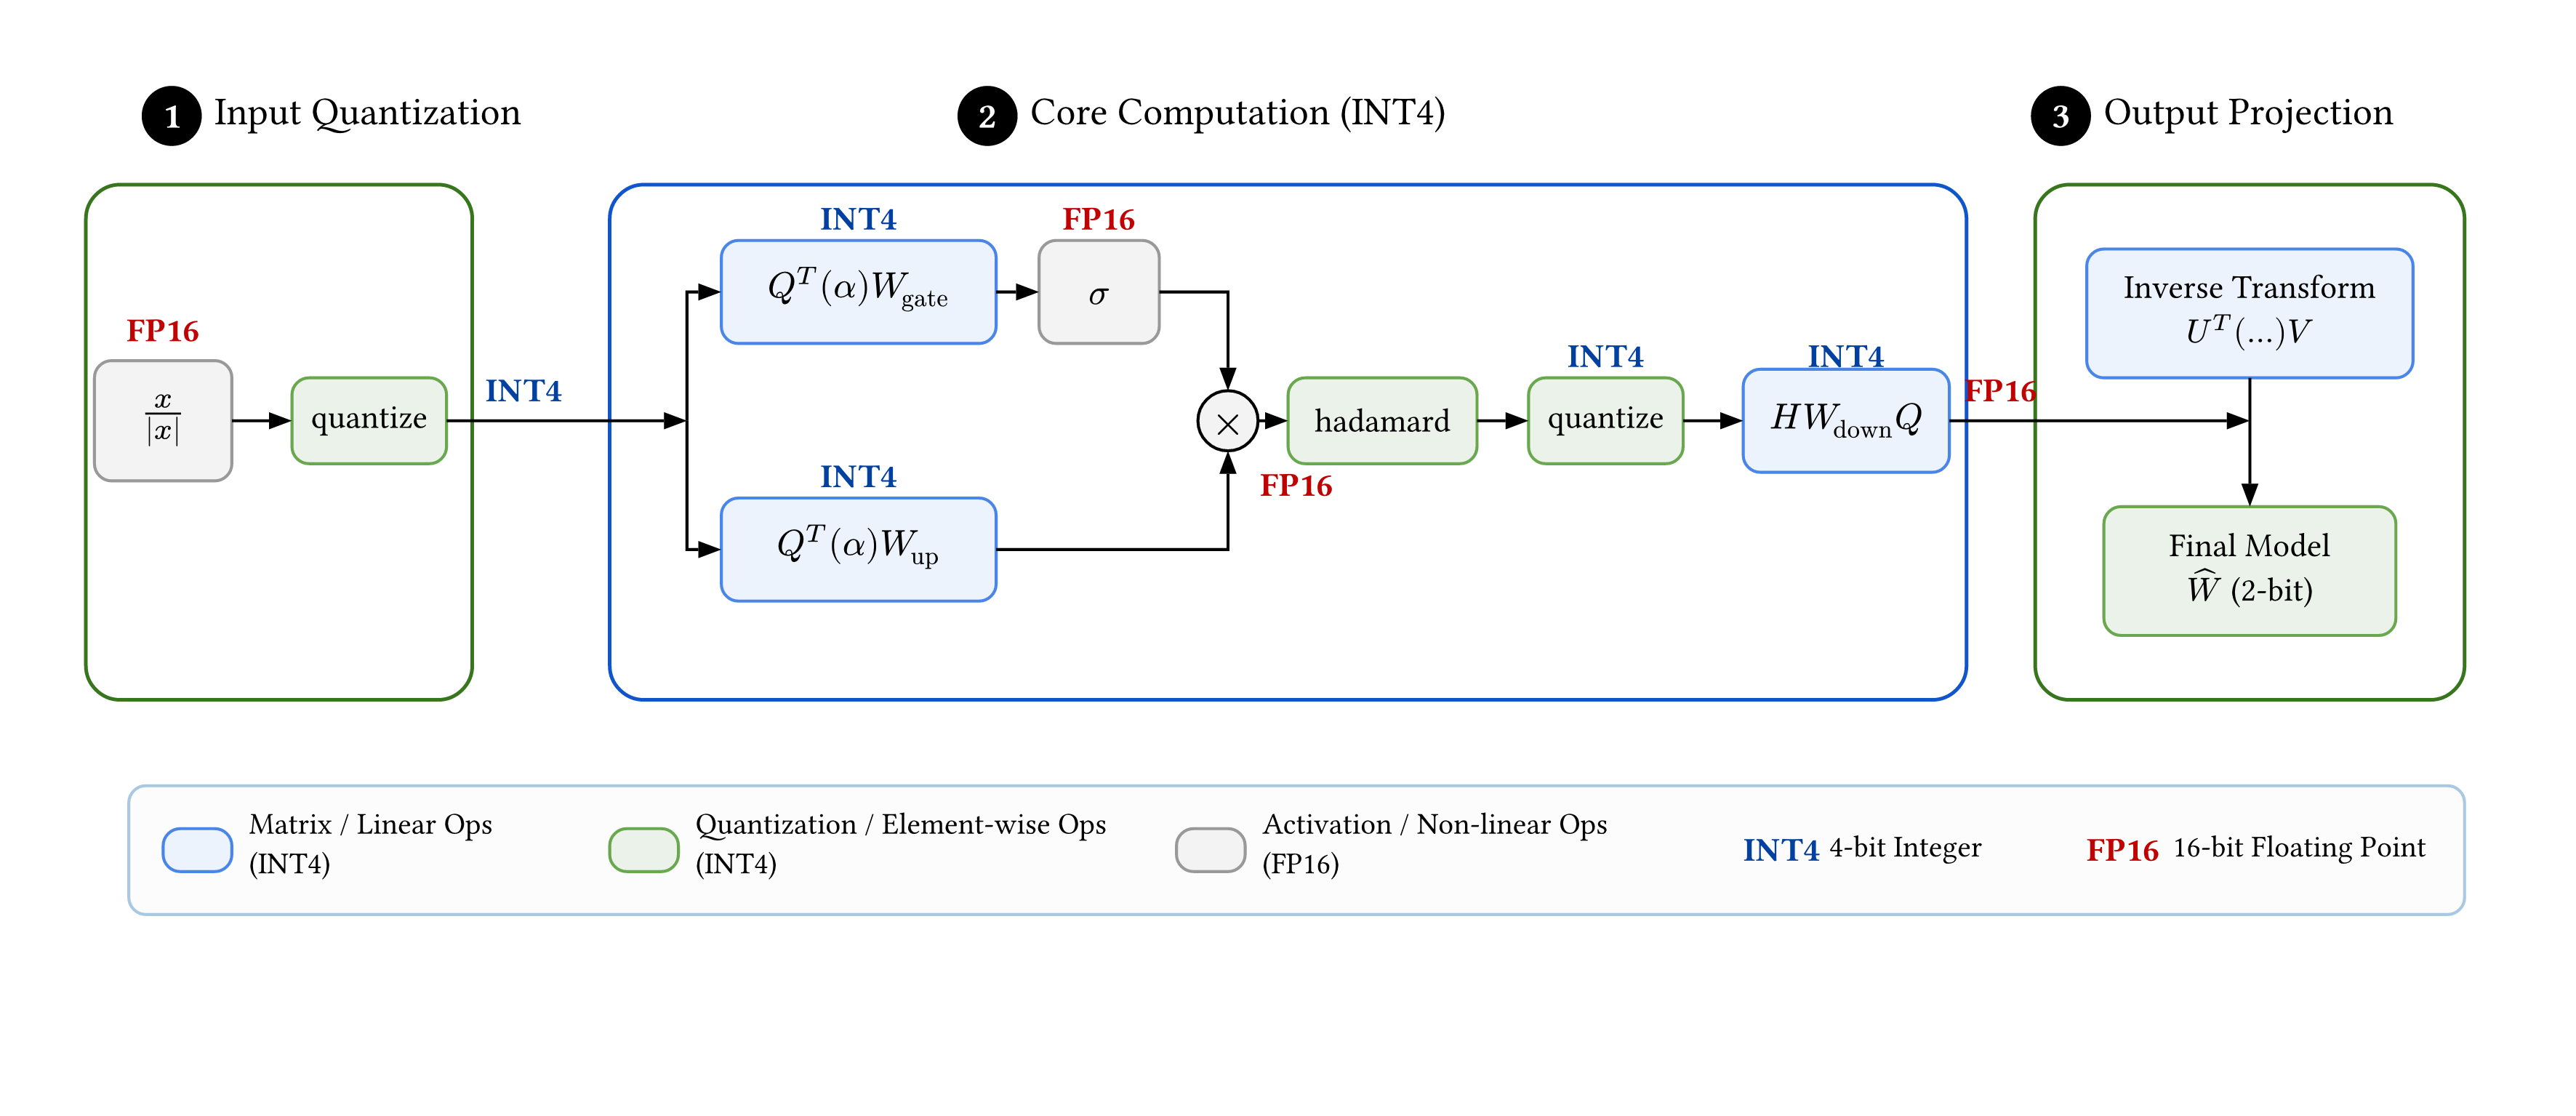
\includegraphics[width=0.98\textwidth,height=0.72\textheight,keepaspectratio]{figures/compression/quarot_pipeline.png}%
  }
  \caption[QuaRot FFN quantization pipeline]{QuaRot applied to a LLaMa-style FFN. RMSNorm scaling ($\alpha$) is absorbed into the weights. Hidden state $X$ is rotated by $Q$, canceled by $Q^\top$ in the first two weights. Weights and activations are INT4; matmul yields INT32, cast and scaled to FP16. While in FP16, a Hadamard transform is applied before quantizing and computing a modified down-proj, producing rotated output $YQ$. \cite{ashkboos2024quarot}}
  \label{fig:quarot}
\end{figure}

QuaRot introduces a quantization scheme based on randomized Hadamard rotations that eliminates activation outliers, enabling true end-to-end 4-bit quantization of weights, activations, and the KV cache (W4A4KV4) without performance degradation. While previous methods rely on mixed-precision inference or complex calibration procedures that introduce computational overhead, QuaRot achieves full 4-bit integer arithmetic by systematically removing the root cause of quantization difficulty.

\paragraph{Methodology.}
The method operates through a two-phase process grounded in the principle of \textit{computational invariance}: transformer weights and activations can be transformed by an orthogonal matrix $\bm{Q}$ without affecting model output, provided the transformation commutes with normalization layers. Specifically, for RMSNorm:
\begin{equation}
  \text{RMSNorm}(\bm{X}) = \text{RMSNorm}(\bm{X}\bm{Q}^\top)\bm{Q}
\end{equation}

\textbf{Phase 1: Rotations via Computational Invariance.} QuaRot fuses randomized Hadamard transformations into model weights to rotate the activation space. The process unfolds in four stages:

\textit{Stage 1a: Global Rotation.} The RMSNorm scaling parameters $\bm{\alpha}$ are absorbed into adjacent weight matrices, and a randomized Hadamard matrix $\bm{Q}$ rotates the hidden state. For input weight matrices (e.g., $\bm{W}_k, \bm{W}_q$):
\begin{equation}
  \bm{W}_{in} \leftarrow \bm{Q}^\top \text{diag}(\bm{\alpha}) \bm{W}_{in}
\end{equation}
Consequently, activations between blocks become $\bm{X} \leftarrow \bm{X}\bm{Q}$.

\textit{Stage 1b: FFN Activation Rotation.} Within the Feed-Forward Network, a Hadamard transformation $\bm{H}$ is inserted on-the-fly and fused into the down-projection:
\begin{equation}
  \bm{W}_{\text{down}} \leftarrow \bm{H} \bm{W}_{\text{down}}
\end{equation}

\textit{Stages 1c \& 1d: Attention and KV Cache.} Hadamard transformations are applied to attention heads to remove outliers from Keys and Values. For value projection $\bm{W}_v$ and output projection $\bm{W}_{\text{out}}$, with head dimension $d_h$:
\begin{equation}
  \bm{W}_v \leftarrow \bm{W}_v (\bm{I} \otimes \bm{H}_{d_h}), \quad \bm{W}_{\text{out}} \leftarrow (\bm{I} \otimes \bm{H}_{d_h}) \bm{W}_{\text{out}}
\end{equation}

\textbf{Phase 2: Quantization.} With outliers eliminated through rotation, the model undergoes quantization:
\begin{itemize}
\item \textbf{Weights:} Quantized using GPTQ or Round-to-Nearest (RTN) to 4 bits
\item \textbf{Activations:} Quantized on-the-fly using symmetric per-token quantization
\item \textbf{KV Cache:} Quantized using asymmetric group-wise quantization
\end{itemize}

\paragraph{Key Properties and Results.}
QuaRot reports strong results. It enables simultaneous 4-bit quantization of weights, activations, and KV cache, yielding up to $3.33\times$ speedup in prefill and $3.89\times$ memory savings during decoding on Llama-2-70B. The rotation-induced "outlier-free" distribution reduces activation quantization error, with the 4-bit Llama-2-70B model retaining 99\% of zero-shot performance and minimal perplexity degradation (0.47 increase on WikiText-2). At higher bit-widths (6-bit, 8-bit), the method reports lossless quantization using simple RTN without requiring calibration data.

\subsubsection{QuIP \cite{chee2024quip}}

\begin{figure}[H]
\centering
\makebox[\textwidth][c]{%
  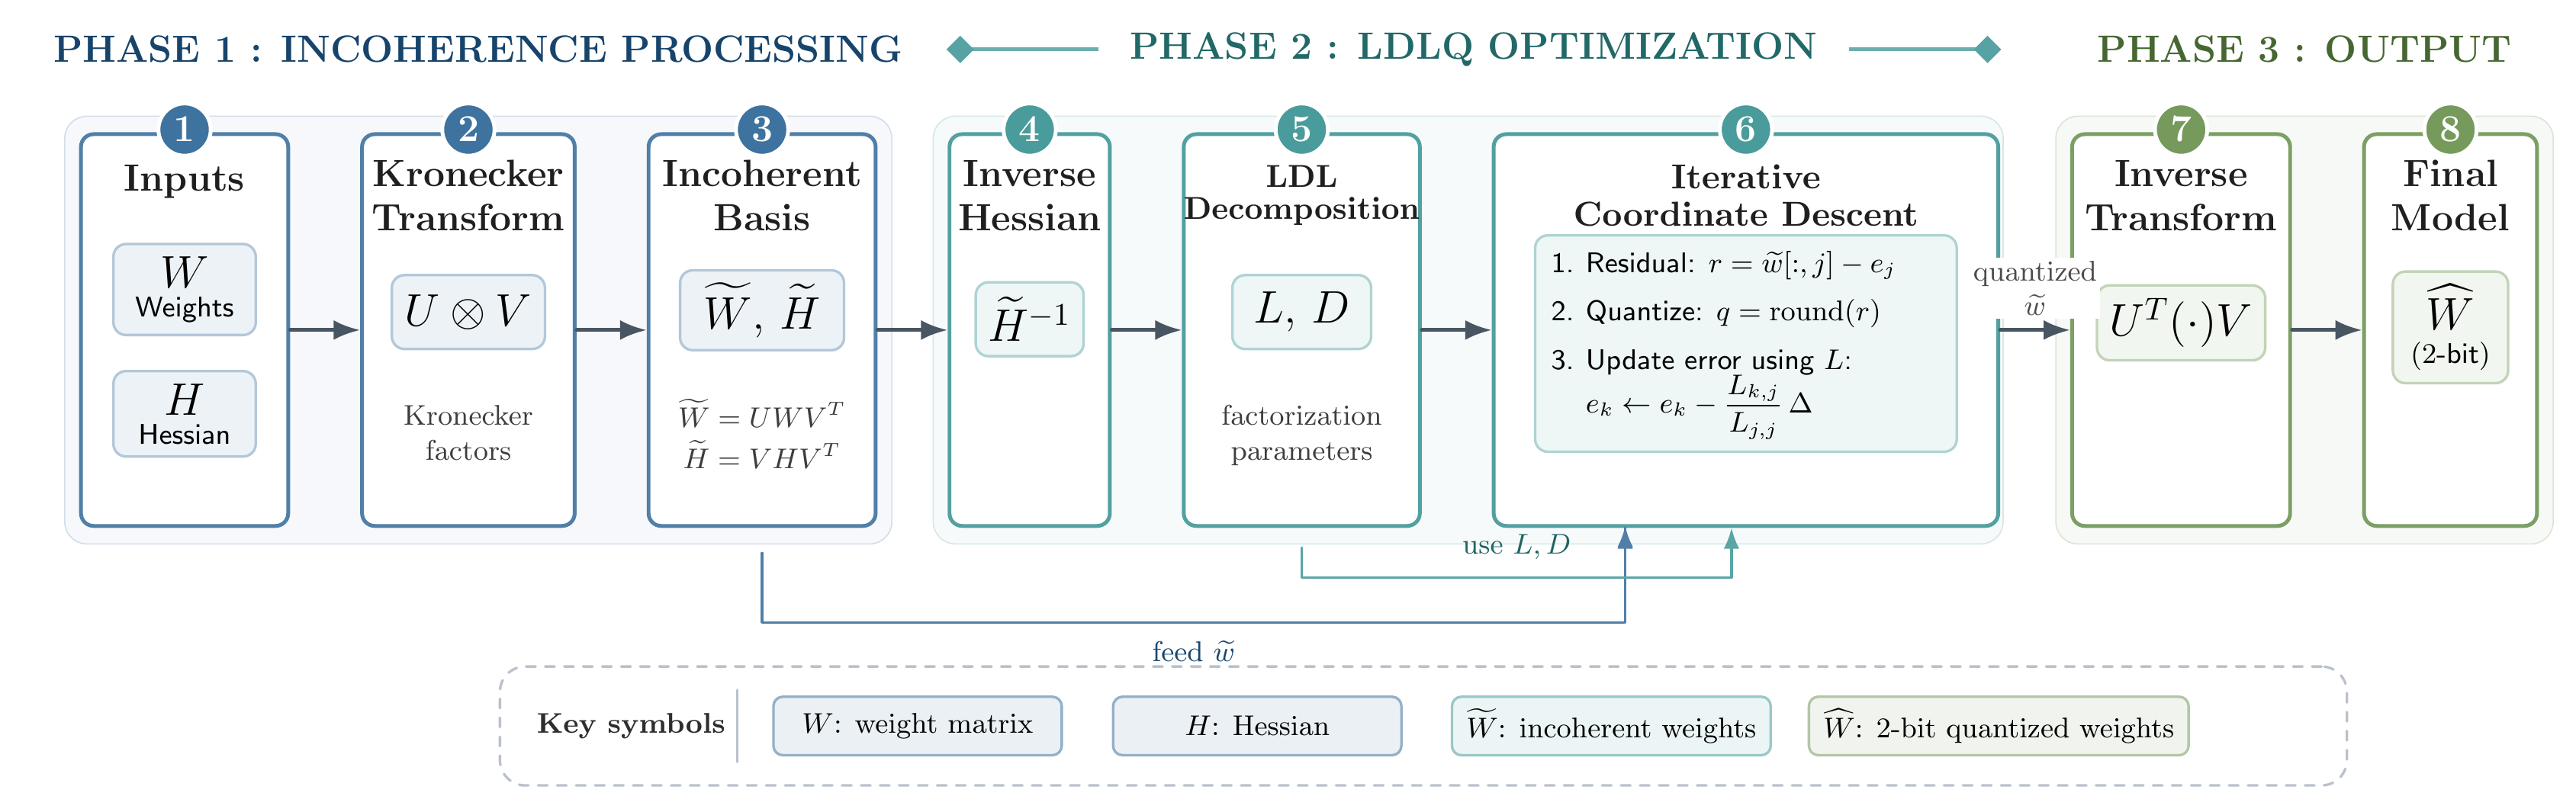
\includegraphics[width=0.98\textwidth,height=0.72\textheight,keepaspectratio]{figures/compression/quip_methodology.png}%
}
\caption[QuIP methodology]{QuIP Methodology. The approach tackles the "proxy gap" in 2-bit quantization by transforming the Hessian and weights into an incoherent basis using Kronecker-factored orthogonal matrices ($U$ and $V$), then employing LDLQ, a coordinate-descent algorithm using the $LDL^T$ decomposition of the inverse Hessian, to quantize weights while correcting errors in remaining full-precision weights. \cite{chee2024quip}}
\label{fig:quip_architecture}
\end{figure}

QuIP addresses the breakdown of conventional quantization proxies at extremely low bit-widths (2 bits) by combining theoretical analysis of incoherence with a novel second-order optimization algorithm. While existing Post-Training Quantization (PTQ) methods like GPTQ minimize a layer-wise quadratic proxy loss that correlates well with task loss at 4 bits, this correlation fails catastrophically at 2 bits, a phenomenon termed the "proxy gap." The root cause lies in the highly coherent Hessian of LLMs, where a few large eigenvalues dominate, causing greedy quantization to yield worst-case $O(N)$ errors as error vectors align with principal eigendirections.

\paragraph{Methodology.}
QuIP provides the first theoretical framework proving that quantization error can be bounded by controlling the incoherence of weight and Hessian matrices. The method consists of three tightly coupled components:

\textbf{1. Incoherence via Orthogonal Transformation.} The quadratic proxy is transformed to "whiten" the optimization landscape. Given input $\bm{X}$ and weights $\bm{W}$:
\begin{equation}
\min_{\hat{\bm{W}}} \|\bm{W}\bm{X} - \hat{\bm{W}}\bm{X}\|_2^2 \implies \min_{\hat{\bm{W}}} \text{Tr}((\tilde{\bm{W}} - \hat{\tilde{\bm{W}}})^\top \tilde{\bm{H}} (\tilde{\bm{W}} - \hat{\tilde{\bm{W}}}))
\end{equation}
Weights and Hessian are transformed via random orthogonal matrices $\bm{U}$ and $\bm{V}$:
\begin{equation}
\tilde{\bm{W}} = \bm{U}\bm{W}\bm{V}^\top, \quad \tilde{\bm{H}} = \bm{V}\bm{H}\bm{V}^\top
\end{equation}
Here, $\bm{V}$ spreads the Hessian's singular values (inducing well-conditioning), while $\bm{U}$ flattens weight magnitude distributions. Both matrices are constructed using Kronecker products of Hadamard matrices, ensuring $O(d \log d)$ multiplication complexity.

\textbf{2. LDLQ Algorithm.} QuIP introduces LDLQ, an iterative coordinate-descent algorithm that exploits the Cholesky decomposition of the inverse Hessian. Let $\bm{H}^{-1} = \bm{L}\bm{D}\bm{L}^\top$. The algorithm iterates through weights $j = 1 \dots d$:
\begin{itemize}
\item Calculate residual error from previously quantized columns
\item Quantize element $\tilde{w}_{j}$ based on diagonal $\bm{D}_{jj}$ and accumulated error
\item Propagate quantization error $\delta_j$ to future columns $k > j$ via:
  \begin{equation}
    \tilde{w}_k \leftarrow \tilde{w}_k - \frac{\bm{L}_{kj}}{\bm{L}_{jj}} \delta_j
  \end{equation}
\end{itemize}
This is equivalent to Optimal Brain Surgeon but implemented efficiently through the fixed $\bm{L}$ decomposition.

\textbf{3. Theoretical Guarantee.} QuIP proves that for block size $n$, if the Hessian and weights are sufficiently incoherent, the proxy loss decreases at rate:
\begin{equation}
\text{Loss} \le O\left(\frac{1}{n}\right) \cdot \mathbb{E}[\text{RoundOffError}]
\end{equation}
This bound ensures that with adequate block sizes and proper incoherence processing, 2-bit quantization error remains bounded rather than diverging.

\paragraph{Key Properties and Results.}
QuIP achieves several critical advances over prior methods. While GPTQ uses Cholesky on $\bm{H}$, LDLQ operates on $\bm{H}^{-1}$; combined with incoherence transforms, this prevents outlier columns from corrupting subsequent quantizations. The Kronecker-structured Hadamard matrices enable scaling to LLaMa-70B without memory explosion ($O(N^2)$ vs $O(N^3)$). Larger quantization block sizes reduce the theoretical error bound, a property unexploited by per-channel methods. Most significantly, QuIP was the first method to generate non-degenerate output for LLaMa-2-70B at 2-bit precision, dramatically outperforming OPTQ and GPTQ which collapse entirely at this regime.

\subsubsection{DuQuant \cite{lin2024duquantdistributingoutliersdual}}

\begin{figure}[H]
\centering
\makebox[\textwidth][c]{%
  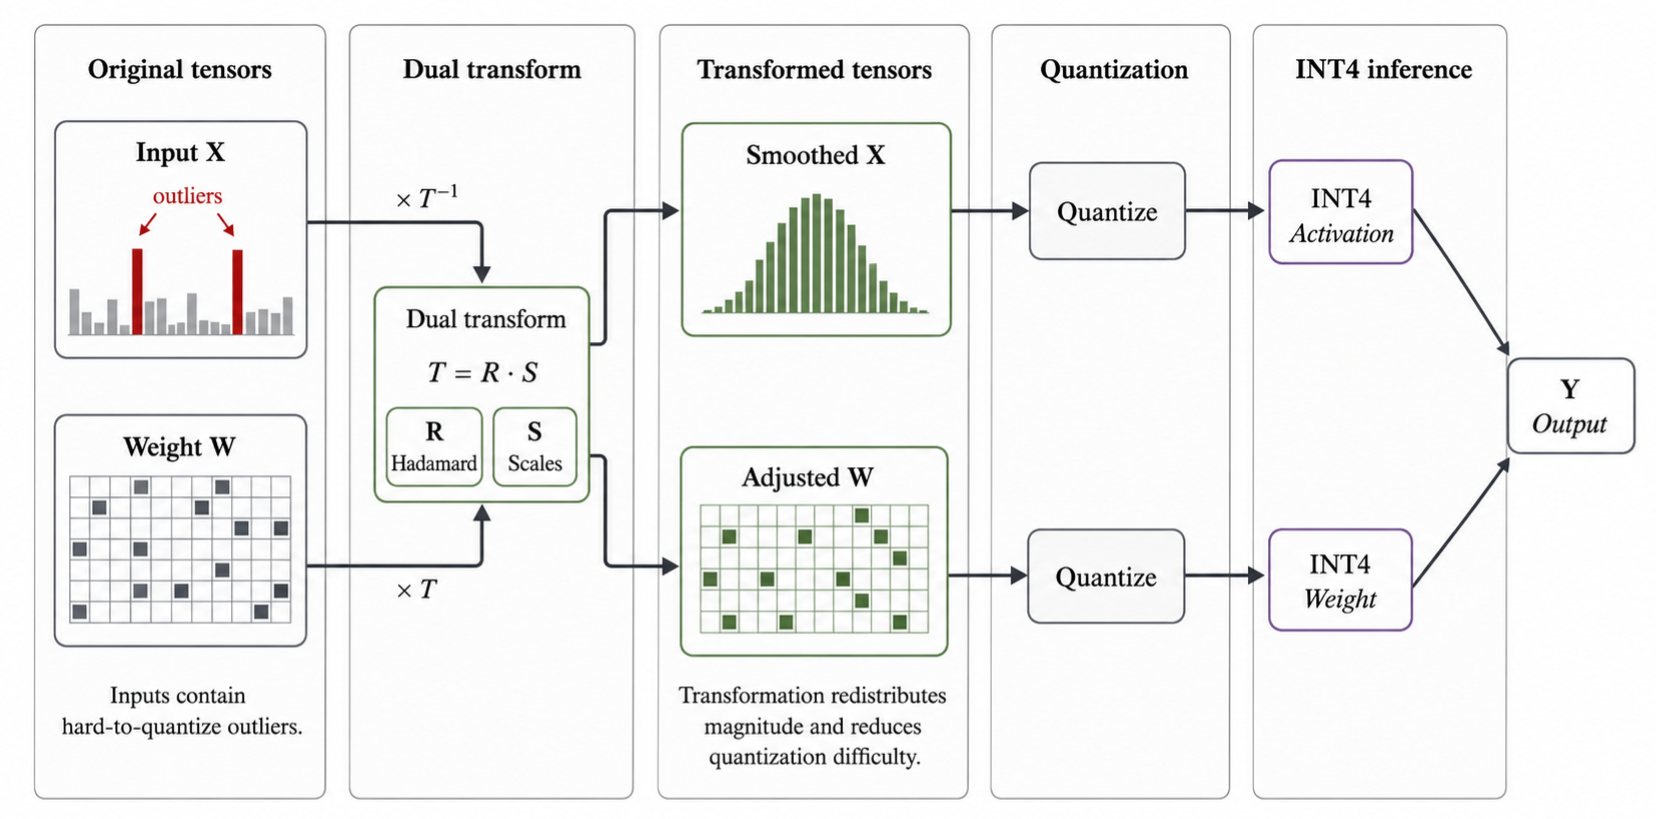
\includegraphics[width=0.72\textwidth,height=0.42\textheight,keepaspectratio]{figures/compression/duquant_pipeline.png}%
}
\caption[DuQuant dual-transformation method]{Overview of the DuQuant dual-transformation method. Unlike QuaRot, which only mixes channels, DuQuant targets massive outliers that survive rotation by applying $\bm{T} = \bm{R} \cdot \bm{S}$, combining orthogonal rotation with learned smoothing to balance weight and activation quantization difficulty. \cite{lin2024duquantdistributingoutliersdual}}
\label{fig:duquant}
\end{figure}

While rotation-based methods like QuaRot successfully mitigate normal outliers by spreading energy across channels, they fail catastrophically on newer architectures (Llama-3, StarCoder2) that exhibit \textit{massive outliers} which are activation channels with magnitudes up to $1000\times$ the median. These extreme outliers persist even after Hadamard rotations because pure rotation redistributes but does not reduce aggregate quantization difficulty. DuQuant addresses this limitation by mathematically fusing rotation with adaptive channel scaling.

\paragraph{Methodology.}
DuQuant proposes a Dual Transformation strategy that combines channel mixing (rotation) with channel scaling (smoothing) into a unified transform $\bm{T}$ that optimally balances the "outlier burden" between weights and activations.

\textbf{Phase 1: Dual Transformation ($\bm{T}$).} For activation $\bm{X}$ and weight $\bm{W}$, the transformation is defined as:
\begin{equation}
\bm{T} = \bm{R} \cdot \bm{S}
\end{equation}
where:
\begin{itemize}
\item $\bm{R}$ (Rotation): Randomized Hadamard Transformations that mix channels, reducing the \textit{number} of outlier channels by delocalizing features
\item $\bm{S}$ (Smoothing): Diagonal scaling matrix that addresses the \textit{magnitude} of massive outliers by scaling down high-variance activation channels while scaling up corresponding weight channels
\end{itemize}

\paragraph{Phase 2: Optimization of Scales.}
Unlike SmoothQuant's heuristic scales, DuQuant derives optimal smoothing scales $\bm{S} = \text{diag}(\bm{s})$ by minimizing combined quantization error:
\begin{equation}
\min_{\bm{s}} \left( \|\bm{X}\text{diag}(\bm{s})^{-1} - Q(\bm{X}\text{diag}(\bm{s})^{-1})\|_F^2 + \lambda \|\text{diag}(\bm{s})\bm{W} - Q(\text{diag}(\bm{s})\bm{W})\|_F^2 \right)
\end{equation}
This convex optimization ensures massive activation outliers are suppressed ($\bm{s}_i > 1$) just enough that increased weight magnitude does not degrade weight quantization.

\textbf{Phase 3: Omni-directional Implementation.} The dual transformation applies to all linear layers and KV Cache. For layer $\bm{Y} = \bm{X}\bm{W}$:
\begin{equation}
  \bm{Y} = (\bm{X}\bm{T}^{-1}) (\bm{T}\bm{W}) \approx Q_{\text{A}}(\bm{X}\bm{T}^{-1}) \cdot Q_{\text{W}}(\bm{T}\bm{W})
\end{equation}

\paragraph{Key Properties and Results.}
DuQuant reports strong performance on newer LLM architectures. It reduces activation kurtosis in Llama-3-70B, converting spiky massive outliers into more Gaussian-like distributions. It is one of the early methods to report successful quantization of Llama-3-70B to W4A4 with negligible performance loss (retaining 98\%+ of FP16 accuracy), where QuaRot typically fails. Ablation studies show that $\bm{R} \cdot \bm{S}$ (Dual) consistently outperforms $\bm{R}$ (rotation alone) and $\bm{S}$ (smoothing alone), indicating that the two operations play complementary roles. The transformations are fused offline, incurring no runtime overhead; inference uses standard INT4 matrix multiplication.

\subsection{Salience-Based Methods}

The fundamental challenge addressed by salience-based methods is the heterogeneous importance of weights within neural networks. Not all parameters contribute equally to model output. Empirical analysis reveals that approximately $1\%$ of weights in Large Language Models are disproportionately critical for performance preservation, while the vast majority exhibit high redundancy. Uniform quantization schemes that apply identical bit-widths across all parameters fail to exploit this structure. They either misallocate precious bits on unimportant weights or catastrophically degrade salient features.

Salience-based approaches address this challenge through precision allocation according to importance. The core principle involves the preservation of high-impact weights with higher precision alongside aggressive quantization of low-impact parameters to minimal bit-widths. The critical technical question becomes: how to accurately measure ``importance'' in a post-train setting without access to gradients or optimization dynamics? Different methods answer this question differently; some rely on activation magnitude analysis, while others utilize Hessian-based sensitivity measures. However, all share the objective to align bit allocation with functional impact.

\subsubsection{AWQ \cite{lin2024awq}}

\begin{figure}[H]
\centering
\makebox[\textwidth][c]{%
  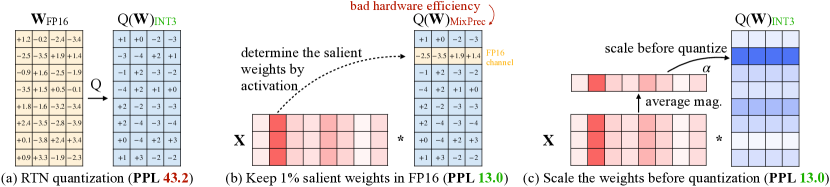
\includegraphics[width=0.98\textwidth,height=0.72\textheight,keepaspectratio]{figures/compression/awq_overview.png}%
}
\caption{Overview of AWQ (Activation-aware Weight Quantization). \cite{lin2024awq}}
\label{fig:awq}
\end{figure}

AWQ (Activation-aware Weight Quantization) challenges the conventional assumption that weight importance correlates with weight magnitude. Through systematic analysis of LLMs, AWQ demonstrates that weight importance is instead determined by the magnitude of the \textit{activation channels} they consume a small fraction $\approx(1\%)$ of salient channels drives the majority of model performance. While existing solutions maintain these critical weights in FP16 (mixed-precision), this approach requires matrix splitting and kernel switching that introduce severe system overhead, negating quantization speedups. AWQ solves this by keeping \textit{all} weights in INT4 while mathematically protecting salient channels through activation-aware scaling.

\paragraph{Methodology.}
AWQ exploits the mathematical invariance of linear layers to scale transformations. For operation $\bm{Y} = \bm{W}\bm{X}$, a channel-wise scaling $\bm{s}$ can be applied:
\begin{equation}
\bm{Y} = \bm{W}\bm{X} = \bm{W}\bm{S} \cdot \bm{S}^{-1}\bm{X} = (\bm{W}\bm{S}) \cdot (\bm{X}\bm{S}^{-1})
\end{equation}
where $\bm{S} = \text{diag}(\bm{s})$.

\textbf{1. Protection via Activation-Aware Scaling.} Since quantization error is bounded by step size $\Delta$, scaling up a salient weight by $s > 1$ reduces relative error:
\begin{equation}
\text{Err}(Q(w \cdot s)) \approx \frac{\Delta}{2} \implies \text{Relative Err} \propto \frac{\Delta}{w \cdot s}
\end{equation}
AWQ "dilates" salient weight channels, allocating them more quantization levels, while compressing non-salient channels.

\textbf{2. Search Space Optimization.} Rather than learning $\bm{s}$ via backpropagation (risking calibration overfitting), AWQ defines a heuristic search based on activation statistics. Let $\bm{s}_X$ be per-channel average activation magnitude. The optimal scale is:
\begin{equation}
\bm{s} = \bm{s}_X^\alpha
\end{equation}
AWQ performs fast grid search over $\alpha \in [0, 1]$ to minimize layer-wise reconstruction error:
\begin{equation}
\min_{\alpha} \left\| \bm{W}\bm{X} - Q(\bm{W} \cdot \text{diag}(\bm{s}_X^\alpha)) \cdot (\text{diag}(\bm{s}_X^{-\alpha}) \bm{X}) \right\|_2^2
\end{equation}

\textbf{3. Efficient Inference Framework.} Scaling factor $\bm{S}$ is permanently fused into weights before quantization ($\bm{W}_{int} = Q(\bm{W}\bm{S})$), while inverse scale $\bm{S}^{-1}$ is applied element-wise to activations. Since element-wise operations are memory-bound but computationally cheap, this incurs negligible cost compared to matrix multiplication. The result is pure INT4 matrix multiplication without mixed-precision complexity.

\paragraph{Key Properties and Results.}
AWQ demonstrates superior calibration robustness compared to GPTQ's Hessian-based approach, which often overfits to calibration data. The heuristic search preserves generalization on instruction-tuned models (e.g., Vicuna) where other methods degrade. The specialized W4A16 CUDA kernel avoids global memory dequantization by performing dequantization in registers, yielding $1.45\times$ speedup over GPTQ-triton. Performance-wise, AWQ achieves perplexity comparable to FP16 on LLaMA-65B and outperforms RTN and GPTQ on zero-shot tasks (MMLU, BoolQ), particularly in low-bit regimes and with small calibration sets.

\subsubsection{OWQ \cite{lee2024owq}}

\begin{figure}[htbp]
\centering
\makebox[\textwidth][c]{%
  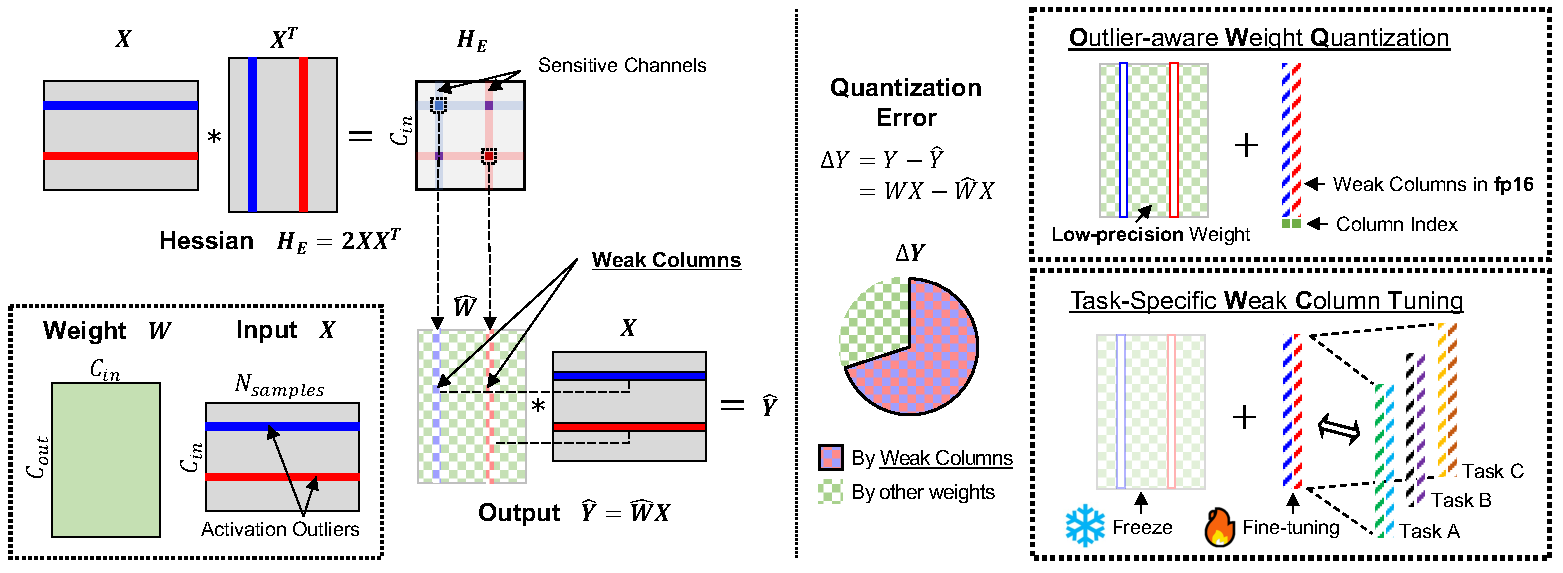
\includegraphics[width=0.98\textwidth,height=0.72\textheight,keepaspectratio]{figures/compression/owq_overview.pdf}%
}
\caption[OWQ overview]{Overview of OWQ (Outlier-Aware Weight Quantization). The method identifies "weak columns" in weight matrix $\bm{W}$ corresponding to outlier activation channels. These columns are segregated into sparse FP16 matrix $\bm{W}_{\text{weak}}$, while remaining "strong columns" are quantized to low precision using GPTQ. \cite{lee2024owq}}
\label{fig:owq}
\end{figure}

OWQ addresses the amplification problem inherent in quantizing weights that interact with outlier activations. Since output error is defined by $\Delta \bm{Y} = \Delta \bm{W} \bm{X}$, when $\bm{X}$ contains channels with magnitudes $100\times$ larger than surrounding features, even small weight quantization errors $\Delta \bm{W}$ in corresponding columns are amplified dramatically. Standard methods either clip activations (permanently destroying information needed for difficult reasoning) or apply uniform quantization (causing performance collapse). OWQ provides a principled mixed-precision solution based on Hessian sensitivity analysis.

\paragraph{Methodology.}
OWQ formulates weight importance through the expected output error variance:
\begin{equation}
\min_{\hat{\bm{W}}} \mathbb{E}\left[ \| (\bm{W} - \hat{\bm{W}})\bm{X} \|_2^2 \right] = \text{Tr}\left( (\bm{W} - \hat{\bm{W}})^\top (\bm{W} - \hat{\bm{W}}) \mathbb{E}[\bm{X}\bm{X}^\top] \right)
\end{equation}
The term $\mathbb{E}[\bm{X}\bm{X}^\top]$ forms the empirical Hessian $\bm{H}$. Error contribution of the $i$-th weight column is proportional to $\bm{H}_{ii}$ (the aggregate power of the $i$-th input feature):
\begin{itemize}
\item \textbf{Weak Columns:} Large $\bm{H}_{ii}$ indicates weights multiplying outlier activations; quantizing them causes high error
\item \textbf{Strong Columns:} Small $\bm{H}_{ii}$ allows aggressive quantization with minimal impact
\end{itemize}

\textbf{Algorithm:}
\begin{itemize}
\item \textit{Step 1: Outlier Selection.} Sort weight columns by Hessian diagonal $\bm{H}_{ii}$; select top-$k$ indices for "weak" set $S_{\text{weak}}$ based on memory budget
\item \textit{Step 2: Matrix Decomposition.} Decompose $\bm{W}$ into:
  \begin{equation}
    \bm{W} = \bm{W}_{\text{quant}} + \bm{W}_{\text{weak}}
  \end{equation}
  where $\bm{W}_{\text{weak}}$ contains FP16 values for $S_{\text{weak}}$ (zeros elsewhere)
\item \textit{Step 3: Quantization.} Apply GPTQ to $\bm{W}_{\text{quant}}$ at low bit-widths (e.g., 3-bit)
\end{itemize}

During inference, matrix multiplication splits into quantized and sparse high-precision paths:
\begin{equation}
\bm{Y} = \text{dequant}(\hat{\bm{W}}_{\text{quant}}) \bm{X} + \bm{W}_{\text{weak}}[\cdot, S_{\text{weak}}] \bm{X}[S_{\text{weak}}, \cdot]
\end{equation}

\paragraph{Key Properties and Results.}
OWQ demonstrates tremendous gains at ultra-low bits: a 3.01-bit OWQ model (3-bit base + 1\% FP16) outperforms standard 4-bit GPTQ in many benchmarks. The work empirically demonstrates that low-bit LLM performance collapse is driven almost entirely by quantization error in the tiny fraction of weight columns corresponding to activation outliers. As a pure PTQ method, OWQ requires only small calibration sets without expensive fine-tuning. It provides Pareto-efficient trade-offs between model size and perplexity, effectively allocating "bit budget" where Hessian analysis indicates maximum necessity.

\subsection{Compensation-Based Methods}

Compensation-based methods address quantization error through corrective updates to unquantized weights. These approaches utilize second-order curvature information to minimize output perturbations. The fundamental challenge stems from greedy quantization, which rounds each weight to the nearest discrete level. This independent operation neglects the interdependencies between parameters. Upon quantization of a weight, the resultant error propagates through the layer computation and influences the optimal values for all subsequent weights. Failure to account for these cross-weight dependencies results in error accumulation that scales poorly with model size, particularly within low-bit regimes.

The critical insight behind compensation-based approaches posits that the \textit{Hessian} (second-order derivative) of the layer-wise reconstruction loss reveals the impact of quantization errors on the optimal values of other weights. Through decomposition of the Hessian (or its inverse) and application of this structure to propagate corrections, these methods transform naive greedy quantization into a globally-aware optimization process. The resultant algorithms achieve superior accuracy-compression trade-offs compared to simple round operations, albeit at the cost of increased computational complexity during the quantization process itself.

\subsubsection{GPTQ \cite{frantar2022gptq}}

\begin{figure}[htbp]
\centering
\makebox[\textwidth][c]{%
  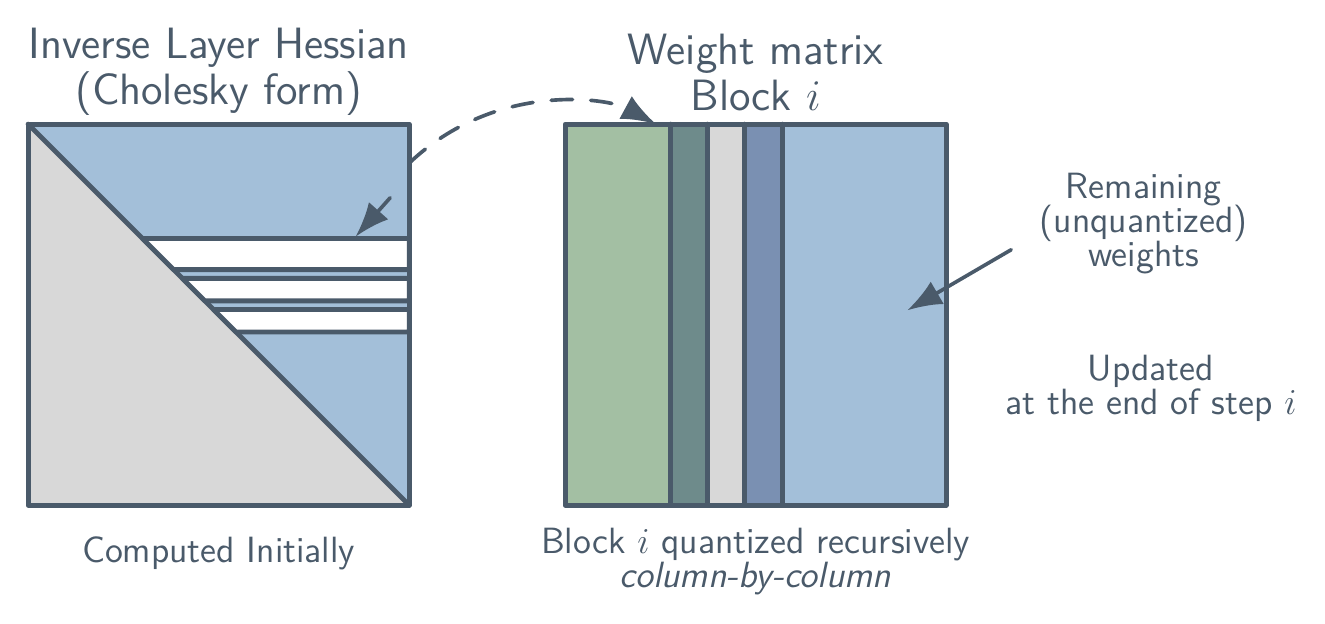
\includegraphics[width=0.98\textwidth,height=0.72\textheight,keepaspectratio]{figures/compression/gptq_pipeline.png}%
}
\caption[GPTQ algorithm]{The GPTQ Algorithm. To avoid computationally prohibitive row-wise updates of OBQ, GPTQ employs a Lazy Batch-Update strategy, quantizing weights in blocks (e.g., 128 columns) with eager intra-block updates and delayed global Hessian updates. \cite{frantar2022gptq}}
\label{fig:gptq}
\end{figure}

GPTQ scales second-order quantization to billion-parameter models by building upon Optimal Brain Quantization (OBQ) while introducing three critical algorithmic innovations that reduce complexity from months to hours. While OBQ provides high-accuracy quantization through Hessian-based error correction, its $O(d_{\text{row}}\cdot d_{\text{col}}^{3})$ complexity renders it infeasible for LLMs. Standard Round-to-Nearest (RTN) executes quickly but destroys accuracy. GPTQ bridges this gap by approximating second-order optimization with runtime comparable to a single forward pass.

\paragraph{Methodology.}
GPTQ solves the layer-wise reconstruction problem:
\begin{equation}
\hat{\bm{W}} \;=\; \arg\min_{\tilde{\bm{W}}} \, \| \bm{W}\bm{X} - \tilde{\bm{W}}\bm{X} \|_{F}^{2}
\end{equation}
Using trace identities, this becomes:
\begin{equation}
\| \bm{W}\bm{X} - \tilde{\bm{W}}\bm{X} \|_{F}^{2} \;=\; \operatorname{Tr}\!\big( (\bm{W}-\tilde{\bm{W}})\,\bm{X}\bm{X}^\top(\bm{W}-\tilde{\bm{W}})^\top \big)
\end{equation}
For a single row $\bm{w}$, the Hessian is $\bm{H} = 2\,\bm{X}\bm{X}^\top$, yielding quadratic form:
\begin{equation}
\ell(\tilde{\bm{w}}) \;=\; \tfrac{1}{2}\,(\bm{w}-\tilde{\bm{w}})^\top \bm{H} (\bm{w}-\tilde{\bm{w}})
\end{equation}

GPTQ introduces three innovations:

\textbf{1. Arbitrary-Order Insight.} OBQ greedily selects the next weight to minimize instantaneous loss increase (per-weight cubic cost). GPTQ observes that fixing a simple column-major order yields negligible accuracy loss for large layers, eliminating expensive sorting while enabling structured updates.

\textbf{2. Cholesky Reformulation.} Rather than repeatedly updating $\bm{H}^{-1}$ (numerically unstable), GPTQ precomputes Cholesky factorization of the damped inverse Hessian:
\begin{equation}
\bm{H}^{-1} \;=\; \bm{L}\bm{L}^\top
\end{equation}
with $\bm{L}$ lower-triangular. This enables stable row extraction and error propagation through triangular factors with better numerical conditioning.

\textbf{3. Lazy Batch-Updates.} Processing columns in blocks of size $B$ (e.g., $B=128$) avoids memory bandwidth bottlenecks. For block indices $Q$, the multi-weight update is:
\begin{align}
\delta_F &= - ( \bm{w}_Q - \operatorname{quant}(\bm{w}_Q) ) \cdot \big( [\bm{H}_F^{-1}]_{QQ} \big)^{-1} \, (\bm{H}_F^{-1})_{:,Q} \\
\bm{H}^{-1}_{-Q} &= \bm{H}^{-1} - \bm{H}^{-1}_{:,Q} \, \big( [\bm{H}^{-1}]_{QQ} \big)^{-1} \, \bm{H}^{-1}_{Q,:}
\end{align}
Intra-block updates use local Cholesky information; once complete, a single global update applies to remaining columns:
\begin{equation}
\bm{W}_{:,(i+B):} \;\leftarrow\; \bm{W}_{:,(i+B):} - \bm{E}\,\bm{H}^{-1}_{\,i:(i+B),\,(i+B):}
\end{equation}
where $\bm{E}$ aggregates per-column quantization errors within the block.

\paragraph{Key Properties and Results.}
GPTQ reduces OBQ runtime by orders of magnitude through shared column ordering, block updates, and Cholesky precomputation. Complexity decreases from $O(d_{\text{row}}\cdot d_{\text{col}}^{3})$ to $O\!\big(\max\{d_{\text{row}}\cdot d_{\text{col}}^{2},\, d_{\text{col}}^{3}\}\big)$ in practice. The method quantizes OPT-175B to 3–4 bits with negligible perplexity degradation in $\approx 4 $  GPU hours (single A100) using 128 calibration samples. It supports flexible bit-widths (4/3/2-bit, with 2-bit typically requiring smaller blocks) and operates as pure post-training quantization requiring minimal calibration data.

\subsubsection{VPTQ \cite{liu2024vptq}}

\begin{figure}[H]
\centering
\makebox[\textwidth][c]{%
  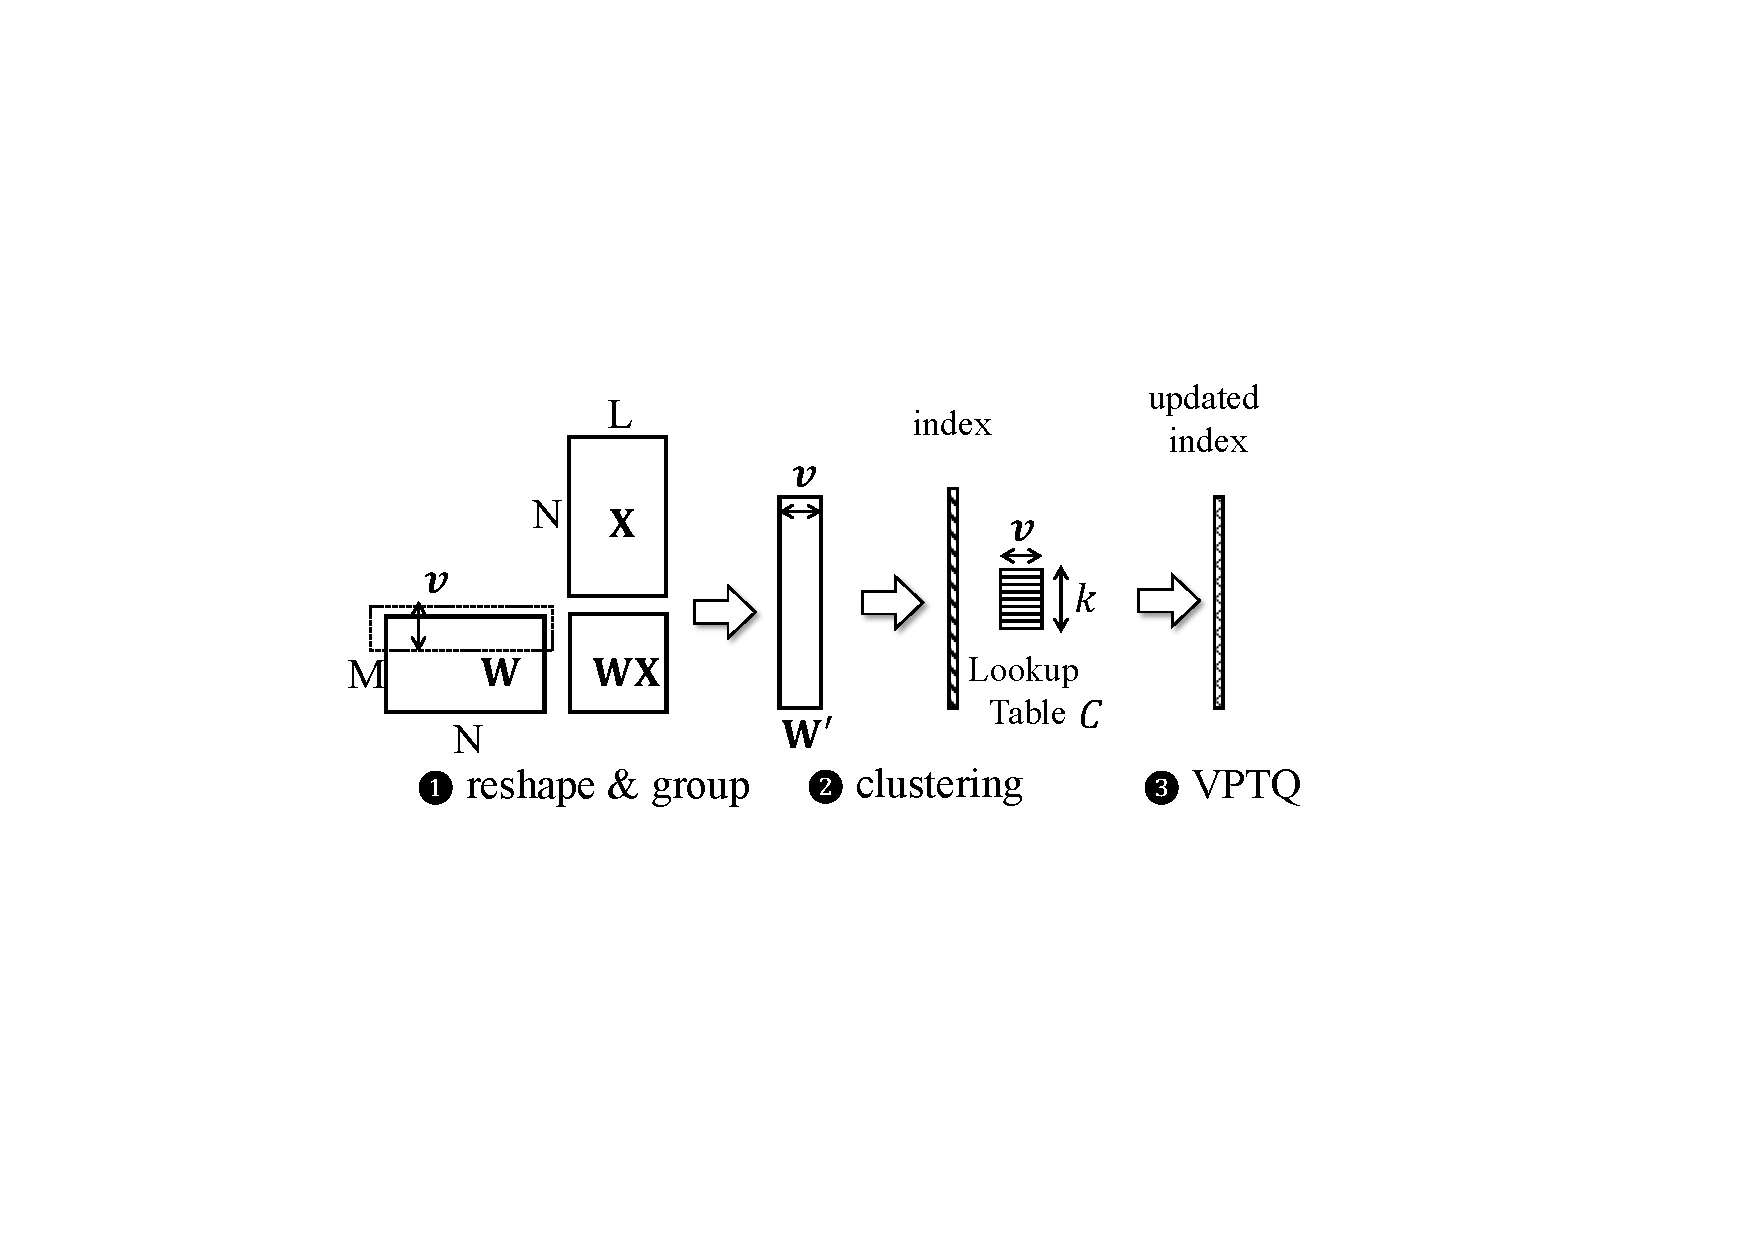
\includegraphics[width=0.72\textwidth,height=0.42\textheight,keepaspectratio]{figures/compression/vptq_methodology.pdf}%
}
\caption[VPTQ methodology]{VPTQ partitions weights into short vectors represented by centroid indices and codebooks. Quantization uses column-wise second-order updates, and inference reconstructs weights through lookup-table reads. \cite{liu2024vptq}}
\label{fig:vptq}
\end{figure}

VPTQ (Vector Post-Training Quantization) targets the regime in which scalar weight-only PTQ becomes unstable, especially near $2$ effective bits. Instead of assigning each scalar weight to one of a few quantized levels, it partitions the weight matrix into short vectors and represents each vector by a centroid index and a codebook entry. This changes the compression unit from an isolated scalar to a local pattern, which permits fractional effective bit-widths and captures correlations among neighboring weights more effectively than scalar rounding. The central problem is then to preserve the second-order PTQ objective while controlling error accumulation during vector assignment and keeping dequantization overhead small \cite{liu2024vptq,frantar2022gptq}.

\paragraph{Methodology.}
Let $\bm{W} \in \mathbb{R}^{d_{\text{out}} \times d_{\text{in}}}$ and let each column be partitioned into vectors $\bm{v}_{j,t} \in \mathbb{R}^{\ell}$ of length $\ell$. With a codebook $\mathcal{C} = \{\bm{c}_1,\dots,\bm{c}_K\}$ and index set $\mathcal{I}$, VPTQ reconstructs each quantized column by concatenating selected centroids. Its starting point is the standard second-order PTQ proxy
\begin{equation}
\min_{\hat{\bm{W}} \in \mathcal{Q}} \operatorname{Tr}\!\big((\bm{W} - \hat{\bm{W}})\,\bm{H}\,(\bm{W} - \hat{\bm{W}})^\top\big),
\end{equation}
where $\bm{H}$ is the layer Hessian surrogate estimated from calibration data and $\mathcal{Q}$ is the set of vector-quantized matrices \cite{liu2024vptq}. The paper's contribution is not merely to replace scalar levels with codebooks, but to redesign the second-order update so that vector quantization remains accurate and efficient in the extreme low-bit regime.

\textbf{1. Channel-Independent Second-Order Quantization.} VPTQ quantizes one matrix column at a time and keeps vector assignment inside that column as the local subproblem. If $\hat{\bm{w}}_j$ denotes the quantized version of column $\bm{w}_j$, the induced error is
\begin{equation}
\bm{\delta}_j = \bm{w}_j - \hat{\bm{w}}_j,
\end{equation}
and the remaining unquantized columns $F$ are updated through
\begin{equation}
\bm{W}_{:,F} \leftarrow \bm{W}_{:,F} - \frac{\bm{\delta}_j}{[\bm{H}^{-1}]_{jj}}[\bm{H}^{-1}]_{jF}.
\end{equation}
This channel-independent formulation is one of the main differences highlighted in the paper. It preserves a GPTQ-like sequential correction while avoiding the larger error accumulation that appears when several columns are quantized jointly \cite{liu2024vptq}.

\textbf{2. Vector Assignment and Codebook Construction.} Once the column-wise second-order update is fixed, each local vector $\bm{v}_{j,t}$ is assigned to the nearest centroid in its codebook:
\begin{equation}
I_{j,t}^{*} = \operatorname*{argmin}_{k \in \{1,\dots,K\}} \|\bm{v}_{j,t} - \bm{c}_{k}\|_2^2.
\end{equation}
The quality of this assignment depends heavily on the initial codebook. Instead of ordinary $k$-means, VPTQ derives a Hessian-weighted initialization from the decomposed second-order proxy:
\begin{equation}
\min_{\mathcal{C},\mathcal{I}} \sum_{j,t} h_{j,t}\,\|\bm{v}_{j,t} - \bm{c}_{I_{j,t}}\|_2^2,
\end{equation}
where $h_{j,t}$ summarizes the local Hessian weight. This gives high-curvature regions a larger influence during centroid construction and improves the starting point for extreme low-bit quantization \cite{liu2024vptq}.

\textbf{3. Residual and Outlier Quantization.} The base vector quantizer is further refined in two ways. First, VPTQ applies residual vector quantization, in which a second codebook compresses the residual left by the first codebook:
\begin{equation}
\bm{r}_{j,t}^{(1)} = \bm{v}_{j,t} - \bm{c}^{(1)}_{I_{j,t}}, \qquad
\bm{r}_{j,t}^{(1)} \approx \bm{c}^{(2)}_{J_{j,t}}.
\end{equation}
Second, it isolates highly sensitive or outlier-dominated tiles and assigns them separate codebooks or partitions. These additions let the method improve accuracy without forcing a single codebook to absorb both normal vectors and highly atypical regions \cite{liu2024vptq}.

\textbf{4. Layer-Wise Refinement and Inference Path.} The end-to-end algorithm quantizes the linear operators of each layer, optionally applies lightweight layer-wise fine-tuning after quantization, and stores the final model as indices plus codebooks. At inference time, the weight matrix is reconstructed by lookup-table reads rather than scalar dequantization arithmetic. The paper emphasizes that throughput then depends strongly on vector length and codebook size, because these determine whether the codebook accesses align well with cache-line and on-chip memory behavior \cite{liu2024vptq}.

\paragraph{Key Properties and Results.}
VPTQ is designed specifically for extreme low-bit weight-only quantization rather than standard 4-bit PTQ. In the EMNLP 2024 paper, it reaches about $2.02$ effective bits on LLaMA-2-7B with WikiText-2 perplexity $6.13$, C4 perplexity $8.07$, average QA accuracy $58.2$, and throughput $39.9$ tok/s; on LLaMA-2-13B it reports $5.32$ WikiText-2 perplexity, $7.15$ C4 perplexity, and $62.4$ average QA at $26.9$ tok/s; and on LLaMA-3-70B it reports about $2.02$ effective bits with WikiText-2 perplexity $5.60$ and average QA $70.9$ \cite{liu2024vptq}. The paper also reports a $1.6\times$ to $1.8\times$ throughput gain over prior ultra-low-bit baselines, attributing this to lookup-based decoding and to vector lengths that better match cache-line granularity. The broader significance of VPTQ is therefore twofold: it shows that vector quantization can remain compatible with second-order PTQ, and it reframes ultra-low-bit compression as a joint problem of numerical approximation and memory-system design.
\subsection{Optimization-Based Methods}

Optimization-based methods reframe post-training quantization as a learnable parameter search problem, replacing hand-crafted heuristics with gradient-based optimization. The core challenge is that conventional PTQ approaches rely on fixed rules for determining quantization parameters: clipping thresholds are set via min-max statistics, scaling factors follow predetermined formulas, and bit allocation uses static heuristics. While computationally efficient, these heuristics are inherently suboptimal: they cannot adapt to layer-specific characteristics, fail to account for inter-parameter dependencies, and often require expensive grid searches over hyperparameters.

The fundamental insight enabling optimization-based approaches is that quantization parameters can be treated as differentiable variables optimized via backpropagation. By freezing the original full-precision weights and instead learning the optimal quantization configuration (clipping bounds, scaling factors, bit allocations), these methods achieve accuracy comparable to Quantization-Aware Training (QAT) while maintaining the computational efficiency of PTQ. The challenge lies in handling the non-differentiable rounding operations inherent in quantization, typically addressed through straight-through estimators that approximate gradients for discrete functions.

\subsubsection{OmniQuant \cite{shao2023omniquant}}

\begin{figure}[htbp]
\centering
\makebox[\textwidth][c]{%
  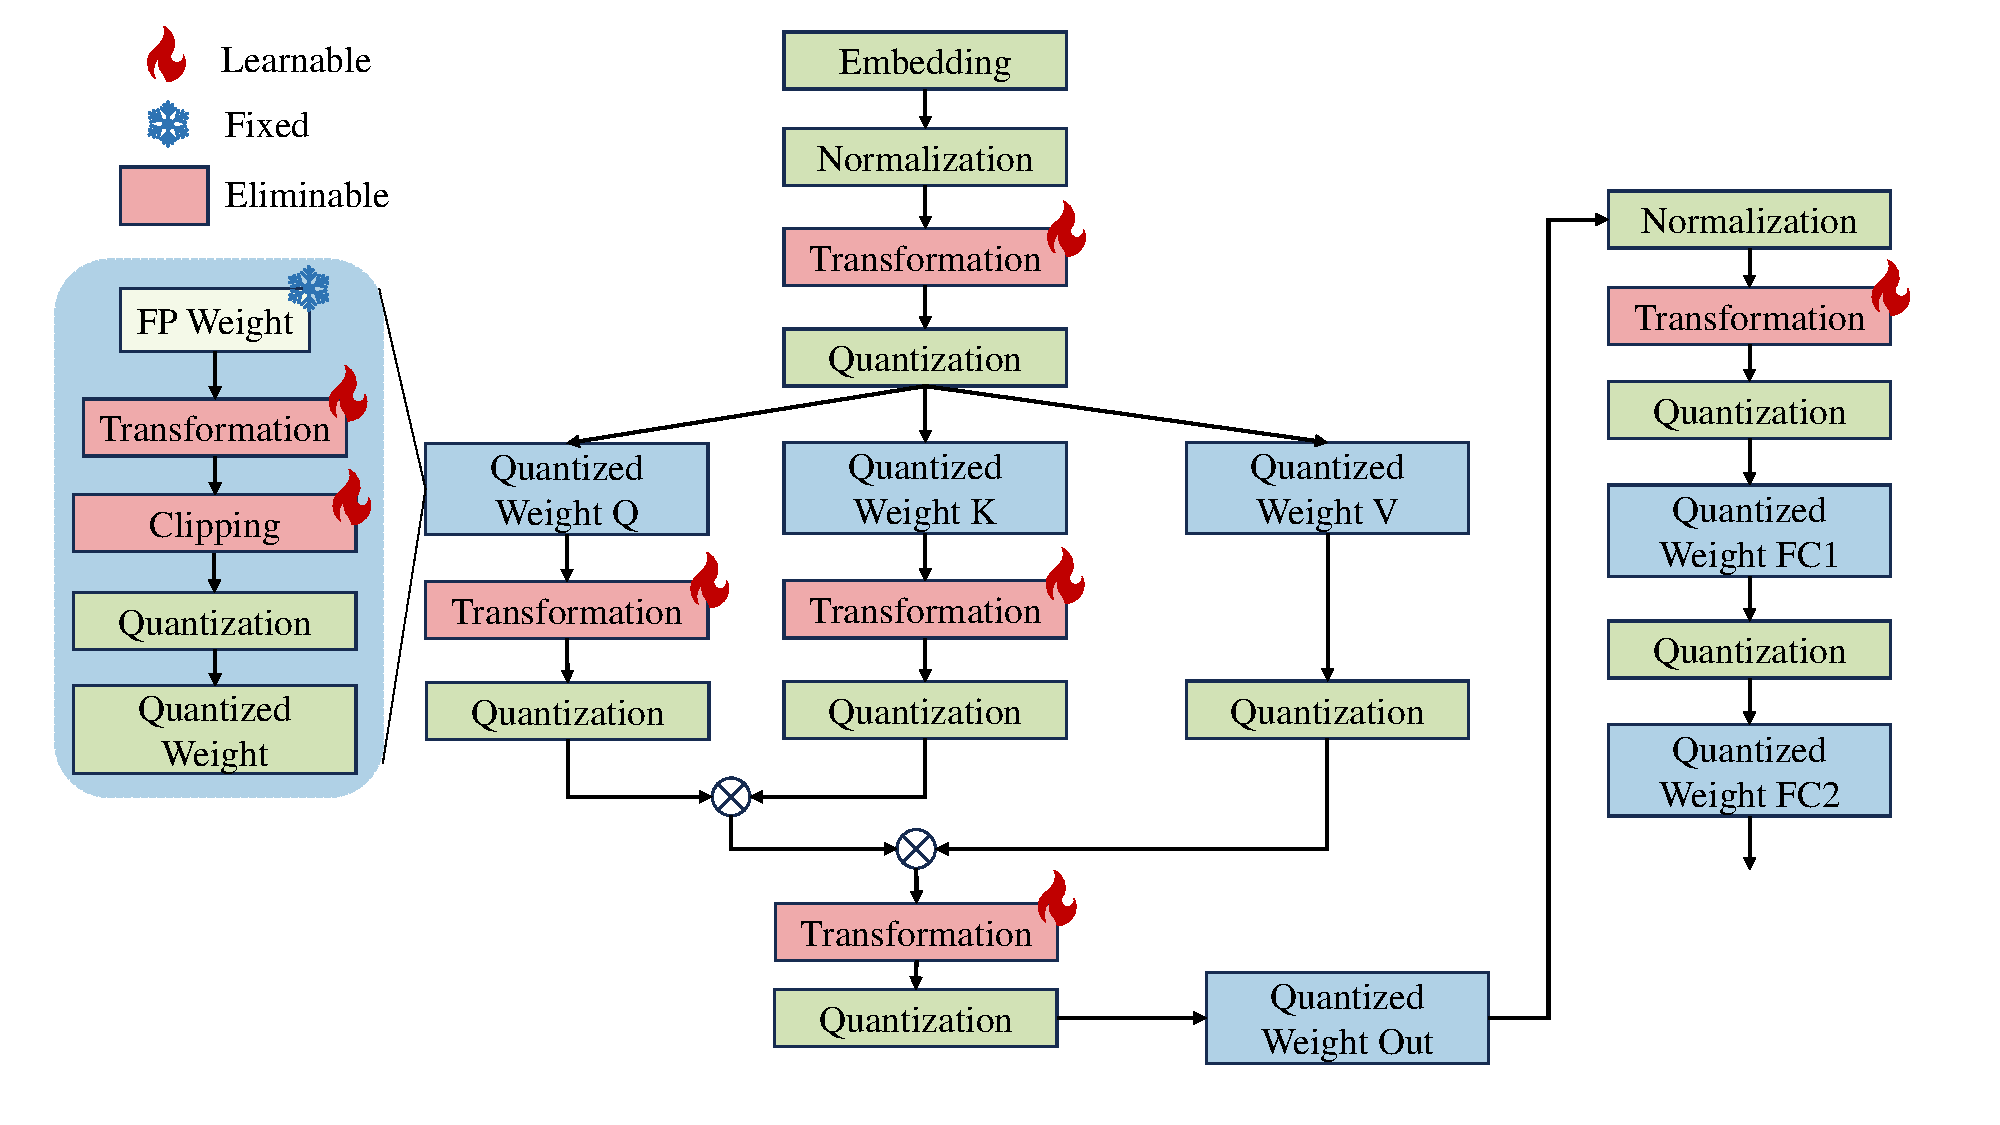
\includegraphics[width=0.98\textwidth,height=0.72\textheight,keepaspectratio]{figures/compression/omniquant_framework.pdf}%
}
\caption[OmniQuant methodology]{OmniQuant Methodology. Unlike PTQ methods relying on hand-crafted heuristics (e.g., SmoothQuant's migration strength $\alpha$) or greedy search (AWQ), OmniQuant freezes original weights and learns quantization parameters via gradient descent, simultaneously optimizing Learnable Weight Clipping (LWC) and Learnable Equivalent Transformation (LET).}
\label{fig:omniquant}
\end{figure}

OmniQuant bridges the gap between the speed of PTQ and the accuracy of QAT through differentiable calibration. While methods like SmoothQuant utilize manually tuned hyperparameters to migrate quantization difficulty from activations to weights, and AWQ employs heuristic grid search over activation statistics, OmniQuant eliminates these design choices by directly optimizing the quantization configuration to minimize layer-wise reconstruction error.

\paragraph{Methodology.}
OmniQuant retains full-precision weights $\bm{W}$ but learns optimal quantization through stochastic gradient descent on loss $\mathcal{L} = \|\bm{Y} - \hat{\bm{Y}}\|_F^2$. The method decomposes quantization difficulty into two learnable operators:

\textbf{1. Learnable Weight Clipping (LWC).} Standard methods clamp weights using static statistics. OmniQuant treats clipping thresholds $[\gamma_l, \gamma_u]$ as learnable parameters:
\begin{equation}
\hat{\bm{W}} = \text{Clamp}\left(\left\lfloor \frac{\bm{W} - \gamma_l}{s_w} \right\rceil \cdot s_w + \gamma_l, \gamma_l, \gamma_u\right), \quad s_w = \frac{\gamma_u - \gamma_l}{2^b - 1}
\end{equation}
Backpropagation through $\gamma_l$ and $\gamma_u$ allows the model to dynamically choose whether to preserve median distribution or accommodate outlier weights based on actual output impact, outperforming AWQ's heuristic grid-search.

\textbf{2. Learnable Equivalent Transformation (LET).} For activation outliers (essential for W4A4), OmniQuant learns channel-wise scaling $\bm{s}$:
\begin{equation}
\bm{Y} = \bm{X}\bm{W}^\top = (\bm{X} \cdot \text{diag}(\bm{s})) (\text{diag}(\bm{s})^{-1} \bm{W}^\top)
\end{equation}
Unlike SmoothQuant's fixed formula $s_j = \max(|X_j|)^\alpha / \max(|W_j|)^{1-\alpha}$, OmniQuant treats $\bm{s}$ as free parameters optimized alongside LWC bounds, learning optimal per-channel migration rather than relying on global assumptions.

\textbf{3. Block-wise Optimization.} For each transformer block, original weights freeze while parameters $\Theta = \{ \gamma_l, \gamma_u, \bm{s} \}$ update via:
\begin{equation}
\Theta^* = \operatorname*{argmin}_{\Theta} \mathbb{E}_{\bm{X}} \left[ \| \text{Block}(\bm{X}) - \text{QuantBlock}(\bm{X}; \Theta) \|_F^2 \right]
\end{equation}
The Straight-Through Estimator (STE) handles non-differentiable rounding $\lfloor \cdot \rceil$, propagating gradients to clipping bounds and scaling factors.

\paragraph{Key Properties and Results.}
OmniQuant eliminates manual hyperparameter tuning, replacing heuristics with gradient descent. It enables effective W4A4 quantization on Llama-2 models where standard PTQ fails due to activation outliers. Learned transformations (LET) fuse into weights and activation quantization parameters offline; inference uses standard quantized matrix multiplication without additional runtime operators. The method works seamlessly for both Weight-Only (W4A16) and Weight-Activation (W4A4) settings, consistently outperforming GPTQ and SmoothQuant in perplexity (e.g., LLaMA-30B W4A16: 7.21 vs 7.64 for GPTQ).

\subsubsection{LRQuant \cite{zhao2024lrquant}}

\begin{figure}[htbp]
    \centering
    \scalebox{0.6}{
    \resizebox{\textwidth}{!}{%
    \begin{tikzpicture}[
        node distance=1cm and 0.5cm,
        box3d/.style={
            rectangle,
            draw=black, thick,
            fill=#1!50,
            minimum width=0.9cm,
            minimum height=1.4cm,
            align=center,
            font=\small\bfseries,
            inner sep=2pt,
            append after command={
                \pgfextra{
                    \begin{pgfonlayer}{background}
                        \filldraw[draw=black, thick, fill=#1!30]
                            (\tikzlastnode.north west) -- ++(0.4,0.3) -- ++(0.93,0) -- (\tikzlastnode.north east) -- cycle;
                        \filldraw[draw=black, thick, fill=#1!70]
                            (\tikzlastnode.north east) -- ++(0.4,0.3) -- ++(0,-1.43) -- (\tikzlastnode.south east) -- cycle;
                    \end{pgfonlayer}
                }
            }
        },
        arrowBlue/.style={-latex, draw=colBlueBorder, line width=1.5pt},
        arrowOrange/.style={-latex, draw=colOrangeBorder, line width=1.5pt},
        arrowBlack/.style={-latex, draw=black, thick},
        labelNode/.style={font=\bfseries, align=center},
        lossCircle/.style={circle, draw=black, thick, fill=gray!30, inner sep=1pt, font=\scriptsize\bfseries, minimum size=0.8cm}
    ]

    \node[labelNode] (fp_title) at (2.5, 4) {Full-Precision Model};
    \node[box3d=colBlue] (fp1) at (0, 2.5) {1\textsuperscript{st}\\Blk};
    \node[box3d=colBlue, right=0.8cm of fp1] (fp2) {2\textsuperscript{nd}\\Blk};
    \node[right=0.2cm of fp2, font=\Large, text=colBlueBorder] (fp_dots) {$\cdots$};
    \node[box3d=colBlue, right=0.2cm of fp_dots] (fp3) {Last\\Blk};
    \draw[arrowBlue] (fp1) -- (fp2);
    \draw[arrowBlue] (fp2) -- (fp_dots);
    \draw[arrowBlue] (fp_dots) -- (fp3);
    \draw[arrowBlue] (fp3.east) -- ++(0.6,0);
    \node[labelNode, left=0.8cm of fp1, font=\footnotesize] (calib1) {Calibration\\Data};
    \draw[arrowBlue] (calib1) -- (fp1);

    \node[rounded corners=15pt, fill=bgYellow, draw=black, thick, minimum width=8.5cm, minimum height=4.0cm] (qbox) at (1.5, -1) {};
    \node[below=0.1cm of qbox.north, font=\bfseries] {Quantization};
    \node[box3d=colBlue] (in_fp) at ($(qbox.west)+(1.5, 0.6)$) {FP\\Blk};
    \node[box3d=colOrange] (in_q) at ($(qbox.east)+(-1.5, 0.6)$) {Q\\Blk};
    \draw[arrowBlue] ($(in_fp.west)+(-0.8,0.2)$) -- node[above, font=\scriptsize, black] {Input} ($(in_fp.west)+(0,0.2)$);
    \draw[arrowOrange] ($(in_q.east)+(0.8,0.2)$) -- node[above, font=\scriptsize, black] {Input} ($(in_q.east)+(0,0.2)$);
    \draw[dashed, thick, ->] ($(in_fp.east)+(0,0.2)$) -- ($(in_q.west)+(0,0.2)$);
    \node[lossCircle] (mse) at ($(in_fp.east)!0.5!(in_q.west) + (-0.8, -1.2)$) {MSE};
    \node[lossCircle] (nlc) at ($(in_fp.east)!0.5!(in_q.west) + (0.8, -1.2)$) {NLC};
    \draw[arrowBlue, ->, rounded corners] ($(in_fp.south east)+(0,0.2)$) |- (mse.west);
    \draw[arrowBlue, ->, rounded corners] ($(in_fp.south)+(0.1,0)$) |- ($(mse.south)+(0,-0.3)$) -| (nlc.south);
    \draw[arrowOrange, ->, rounded corners] ($(in_q.south)+(-0.1,0)$) |- ($(nlc.south)+(0,-0.4)$) -| (mse.south);
    \draw[arrowOrange, ->, rounded corners] ($(in_q.south west)+(0,0.2)$) |- (nlc.east);
    \node[red!80!black, font=\bfseries] (thetas) at ($(in_fp.east)!0.5!(in_q.west) + (0, -0.4)$) {$\theta_s, \theta_q$};
    \draw[->, red!80!black, thick] (mse.north) -- (thetas.south west);
    \draw[->, red!80!black, thick] (nlc.north) -- (thetas.south east);
    \draw[arrowBlack] (fp1.south) -- (fp1|-qbox.north);
    \draw[arrowBlack] (fp2.south) -- (fp2|-qbox.north);
    \draw[arrowBlack] (fp3.south) -- ++(0,-0.5) -| ($(qbox.north)+(3,0)$);

    \node[box3d=colOrange] (q1) at (0, -4.5) {1\textsuperscript{st}\\Blk};
    \node[box3d=colOrange, right=0.8cm of q1] (q2) {2\textsuperscript{nd}\\Blk};
    \node[right=0.2cm of q2, font=\Large, text=colOrangeBorder] (q_dots) {$\cdots$};
    \node[box3d=colOrange, right=0.2cm of q_dots] (q3) {Last\\Blk};
    \node[labelNode] at (1, -5.7) {Quantized Model};
    \draw[arrowOrange] (q1) -- (q2);
    \draw[arrowOrange] (q2) -- (q_dots);
    \draw[arrowOrange] (q_dots) -- (q3);
    \draw[arrowOrange] (q3.east) -- ++(0.6,0);
    \draw[arrowBlack] (fp1|-qbox.south) -- (q1.north);
    \draw[arrowBlack] (fp2|-qbox.south) -- (q2.north);
    \draw[arrowBlack] ($(qbox.south)+(3,0)$) |- ++(0,-0.5) -| (q3.north);
    \node[labelNode, left=0.8cm of q1, font=\footnotesize] (calib2) {Calibration\\Data};
    \draw[arrowOrange] (calib2) -- (q1);

    \node[box3d=colBlue] (test_blk) at (7.5, 2.5) {Last\\Blk};
    \node[right=0.6cm of test_blk, font=\footnotesize\bfseries, align=left] (test_data) {Test\\Data};
    \draw[arrowBlue] (test_data) -- (test_blk);
    \node[box3d=colGreen] (new_last) at (7.5, -4.5) {New\\Last\\Blk};
    \draw[arrowBlack, rounded corners] (test_blk.west) -| ($(qbox.east)+(0.3,0.8)$) -- ($(qbox.east)+(-0.08,0.8)$);
    \draw[arrowBlack, rounded corners] ($(qbox.east)+(-0.1,-1.5)$) -- ($(qbox.east)+(0.5,-1.5)$) |- (new_last.west);
    \draw[dotted, thick, colGreen!80!black, ->, out=20, in=160] (fp3.north) to (test_blk.north);
    \draw[dotted, thick, colGreen!80!black, ->, bend left=25] (new_last.south) to (q3.south);
    \node[font=\bfseries, align=center, text=colGreen!50!black] at (8.5, -1) {Test--Time\\Adaptation};

    \begin{scope}[on background layer]
        \fill[bgGray] (-3.4, 5) rectangle (6, -6);
        \draw[gray!40] (-3.4, 5) rectangle (6, -6);
        \fill[bgGreen] (6.2, 5) rectangle (10, -6);
    \end{scope}

    \end{tikzpicture}%
    }}
    \caption{Overview of LRQuant. LRQuant uses NLC loss and MSE loss to update learnable smoothing and quantization parameters. During testing, LRQuant utilizes test data to adapt the last block to improve performance on unseen data.}
    \label{fig:lrquant} 
\end{figure}

LRQuant (Learnable and Robust Quantization) extends optimization-based PTQ by addressing two critical limitations: the reliance on suboptimal static heuristics for smoothing parameters, and poor generalization under distribution shift between calibration and deployment data. While methods like SmoothQuant use hand-crafted formulas for migrating outlier difficulty from activations to weights (e.g., static migration strength $\alpha$), and existing approaches optimize using Mean Squared Error (MSE) which poorly correlates with semantic generation quality, LRQuant introduces an end-to-end differentiable framework with semantic-aware loss and test-time adaptation.

\paragraph{Methodology.}
LRQuant introduces three key innovations for high-fidelity low-bit quantization:

\textbf{1. Learnable Smoothing Paradigm.} Rather than calculating smoothing scales $\mathbf{s}$ from fixed activation statistics, LRQuant defines $\mathbf{s}$ as learnable parameters. The transformation is:
\begin{equation}
\hat{\bm{W}} = \bm{W} \cdot \text{diag}(\mathbf{s})^{-1}, \quad \hat{\bm{X}} = \text{diag}(\mathbf{s}) \cdot \bm{X}
\end{equation}
Parameters initialize using "Logarithmic Activation Equivalent" strategy for stability, then fine-tune via gradient descent to minimize layer output reconstruction error.

\textbf{2. NLC Loss (Negative Log-Cosine).} Recognizing that MSE focuses on element-wise magnitude errors (misleading for LLM generation where token semantics matter more than absolute magnitude), LRQuant employs Negative Log-Cosine similarity loss:
\begin{equation}
\mathcal{L}_{\text{NLC}} = - \log \left( \frac{\bm{Y}_{\text{FP}} \cdot \bm{Y}_{\text{Q}}}{\| \bm{Y}_{\text{FP}} \|_2 \| \bm{Y}_{\text{Q}} \|_2} \right)
\end{equation}
Minimizing $\mathcal{L}_{\text{NLC}}$ maximizes cosine similarity between full-precision output $\bm{Y}_{\text{FP}}$ and quantized output $\bm{Y}_{\text{Q}}$, ensuring token representation vectors point in correct semantic directions.

\textbf{3. Test-Time Adaptation (TTA).} To handle distribution shifts (e.g., calibration data to real-world prompts), LRQuant introduces lightweight inference-time adaptation. For test input batches, the method performs rapid gradient steps on quantization parameters (scales and bias) to minimize discrepancy on current data:
\begin{equation}
\theta_{\text{test}} \leftarrow \theta_{\text{test}} - \eta \nabla_{\theta} \mathcal{L}(\bm{X}_{\text{test}})
\end{equation}
This allows the quantizer to adapt to specific activation outliers in user prompts.

\paragraph{Key Properties and Results.}
LRQuant eliminates manual tuning of smoothing factor $\alpha$, finding mathematically optimal outlier distribution between weights and activations. The robust NLC loss landscape significantly outperforms baselines (SmoothQuant, AWQ) on out-of-distribution datasets. TTA overhead is negligible compared to decoding time but provides consistent perplexity recovery on difficult benchmarks. Performance-wise, LRQuant achieves near FP16 performance on LLaMA and OPT families at W4A8 (4-bit weights, 8-bit activations), effectively solving the "outlier channel" problem without complex mixed-precision arithmetic.

\subsection{Empirical Comparison}


\begin{table}[htbp]
\centering
\begin{tabular}{lcccccc}
  \hline
  & \textbf{PTQ} & \textbf{AQLM} & \textbf{QuIP\#} & \textbf{GPTVQ} & \textbf{GPTQ} & \textbf{AWQ} \\
  \hline
  \textbf{Effective Bitwidth}
  & \textcolor{red}{\(\downarrow\downarrow\downarrow\)}
  & \textcolor{red}{\(\downarrow\)}
  & \textcolor{red}{\(\downarrow\)}
  & \textcolor{green}{\(\uparrow\)}
  & \textcolor{green}{\(\uparrow\uparrow\)}
  & \textcolor{green}{\(\uparrow\uparrow\)} \\

  \textbf{Accuracy @ Low-bit}
  & \textcolor{green}{\(\uparrow\uparrow\uparrow\)}
  & \textcolor{green}{\(\uparrow\)}
  & \textcolor{green}{\(\uparrow\)}
  & \textcolor{red}{\(\downarrow\)}
  & \textcolor{red}{\(\downarrow\downarrow\)}
  & \textcolor{red}{\(\downarrow\downarrow\)} \\

  \textbf{Quantization Time Cost}
  & \textcolor{red}{\(\downarrow\downarrow\downarrow\)}
  & \textcolor{green}{\(\uparrow\uparrow\)}
  & \textcolor{red}{\(\downarrow\)}
  & \textcolor{red}{\(\downarrow\)}
  & \textcolor{red}{\(\downarrow\)}
  & \textcolor{red}{\(\downarrow\)} \\

  \textbf{Inference Throughput}
  & \textcolor{green}{\(\uparrow\uparrow\uparrow\)}
  & \textcolor{green}{\(\uparrow\)}
  & \textcolor{red}{\(\downarrow\)}
  & \textcolor{green}{\(\uparrow\)}
  & \textcolor{green}{\(\uparrow\)}
  & \textcolor{green}{\(\uparrow\)} \\
  \hline
\end{tabular}
\caption{Qualitative comparison of post-training quantization methods.}
\end{table}




\mainp{Modern Weight-Only Quantization (2-4 bits)}
\textit{Comparison across LLaMA-3 and Mistral architectures.}

\begin{table}[htbp]
\centering
\caption{Weight-only performance on LLaMA-3 (8B/70B) and Mistral 7B. (PPL $\downarrow$, Acc $\uparrow$)}
\label{tab:llama3-mistral-merged}
\begin{adjustbox}{max width=\textwidth}
  \begin{tabular}{l|c|cc|cc|ccc}
    \toprule
    & & \multicolumn{2}{c|}{\textbf{LLaMA-3 8B}} & \multicolumn{2}{c|}{\textbf{LLaMA-3 70B}} & \multicolumn{3}{c}{\textbf{Mistral 7B}} \\
    \textbf{Method} & \textbf{Bits} & \textbf{Wiki2} & \textbf{AvgQA} & \textbf{Wiki2} & \textbf{AvgQA} & \textbf{Wiki2} & \textbf{C4} & \textbf{AvgQA} \\
    \midrule
    FP16 & 16.0 & 6.14 & 68.6 & 2.90 & 75.3 & 4.77 & 5.71 & 68.6 \\
    \midrule
    QuIP & 4.0 & 6.50 & 67.1 & 3.40 & 74.5 & 4.85 & 5.79 & 68.7 \\
    GPTQ & 4.0 & 6.50 & 67.3 & 3.30 & 74.9 & 4.83 & 5.74 & 68.4 \\
    VPTQ & $\sim$4.0 & 6.42 & 68.1 & 3.15 & 74.7 & 4.81 & 5.72 & 68.2 \\
    \midrule
    QuIP & 3.0 & 7.50 & 63.7 & 4.70 & 72.6 & 5.07 & 5.97 & 67.3 \\
    GPTQ & 3.0 & 8.20 & 61.7 & 5.20 & 70.6 & 1535$^\dagger$ & 164$^\dagger$ & 44.5$^\dagger$ \\
    VPTQ & $\sim$3.0 & 6.97 & 66.7 & 3.81 & 73.7 & 4.96 & 5.84 & 67.3 \\
    \midrule
    QuIP\# & 2.0 & 85.1 & 36.8 & 13.0 & 48.7 & 6.02 & 6.84 & 62.2 \\
    AQLM & 2.0 & 6.32 & 62.2 & - & - & 6.32 & 6.93 & 62.2 \\
    GPTVQ & 2.25 & 8.99 & 57.7 & - & - & 8.99 & 18.6 & 57.7 \\
    VPTQ & $\sim$2.0 & 5.64 & 63.2 & 5.66 & 70.7 & 5.64 & 6.43 & 63.2 \\
    \bottomrule
    \multicolumn{9}{l}{\footnotesize $^\dagger$ Mistral GPTQ result at 2.125 bits.}
  \end{tabular}
\end{adjustbox}
\end{table}

\mainp{Weight-Only on LLaMA-1 \& LLaMA-2 Families}

\begin{table}[htbp]
\centering
\caption{WikiText2 Perplexity ($\downarrow$) for Weight-Only Quantization on LLaMA-1 and LLaMA-2.}
\label{tab:llama1-2-weight-merged}
\begin{adjustbox}{max width=\textwidth}
  \begin{tabular}{ll|cccc|ccc}
    \toprule
    & & \multicolumn{4}{c|}{\textbf{LLaMA-1}} & \multicolumn{3}{c}{\textbf{LLaMA-2}} \\
    \textbf{Method} & \textbf{Config} & \textbf{7B} & \textbf{13B} & \textbf{30B} & \textbf{65B} & \textbf{7B} & \textbf{13B} & \textbf{70B} \\
    \midrule
    FP16 & - & 5.68 & 5.09 & 4.10 & 3.53 & 5.47 & 4.88 & 3.31 \\
    \midrule
    \multirow{2}{*}{W2A16}
    & GPTQ & 2.1e3 & 5.5e3 & 499.7 & 55.9 & 7.7e3 & 2.1e3 & 77.9 \\
    & OmniQuant & 15.47 & 13.21 & 8.71 & 7.58 & 37.37 & 17.21 & 7.81 \\
    \midrule
    \multirow{2}{*}{W2A16 g128}
    & GPTQ & 44.01 & 15.60 & 10.92 & 9.51 & 36.77 & 28.14 & NaN \\
    & OmniQuant & 9.72 & 7.93 & 7.12 & 5.95 & 11.06 & 8.26 & 6.55 \\
    \midrule
    \multirow{2}{*}{W2A16 g64}
    & GPTQ & 22.10 & 10.06 & 8.54 & 8.31 & 20.85 & 22.44 & NaN \\
    & OmniQuant & 8.90 & 7.34 & 6.59 & 5.65 & 9.62 & 7.56 & 6.11 \\
    \midrule
    \multirow{2}{*}{W3A16}
    & GPTQ & 8.06 & 6.76 & 5.84 & 5.06 & 8.37 & 6.44 & 4.82 \\
    & OmniQuant & 6.49 & 5.68 & 4.74 & 4.04 & 6.58 & 5.58 & 3.92 \\
    \midrule
    \multirow{2}{*}{W3A16 g128}
    & GPTQ & 6.55 & 5.62 & 4.80 & 4.17 & 6.29 & 5.42 & 3.85 \\
    & OmniQuant & 6.15 & 5.44 & 4.56 & 3.94 & 6.03 & 5.28 & 3.78 \\
    \midrule
    \multirow{2}{*}{W4A16}
    & GPTQ & 6.13 & 5.40 & 4.48 & 3.83 & 5.83 & 5.13 & 3.58 \\
    & OmniQuant & 5.86 & 5.21 & 4.25 & 3.71 & 5.74 & 5.02 & 3.47 \\
    \midrule
    \multirow{2}{*}{W4A16 g128}
    & GPTQ & 5.85 & 5.20 & 4.23 & 3.65 & 5.61 & 4.98 & 3.42 \\
    & OmniQuant & 5.77 & 5.17 & 4.19 & 3.62 & 5.58 & 4.95 & 3.40 \\
    \bottomrule
  \end{tabular}
\end{adjustbox}
\end{table}
\newpage
\mainp{Specialized Comparisons (3-bit \& Rotation)}

\noindent\begin{minipage}{0.47\textwidth}
\centering
\captionsetup{hypcap=false}
\captionof{table}{3-bit Weight-Only on OPT-6.7B \& LLaMA-7B.}
\label{tab:3bit-merged}
\resizebox{\textwidth}{!}{
  \begin{tabular}{l|cccc}

    \toprule
    \textbf{OPT-6.7B} & \textbf{Wiki2} & \textbf{PTB} & \textbf{C4} & \textbf{LAMB.} \\
    \midrule
    OPTQ (3b) & 12.76 & 19.35 & 14.55 & 60.15 \\
    OPTQ (3b-g1024) & 12.05 & 18.01 & 13.89 & 64.44 \\
    OPTQ (3b-g128) & 11.55 & 17.26 & 13.43 & 64.96 \\
    OWQ (3.01b) & 11.22 & 16.32 & 13.23 & 69.94 \\
    OWQ (g1024) & 11.18 & 16.32 & 13.19 & 68.91 \\
    OWQ (g128) & 11.16 & 16.23 & 13.10 & 68.61 \\
    \midrule
    \textbf{LLaMA-7B} & \textbf{Wiki2} & \textbf{PTB} & \textbf{C4} & \textbf{Wino.} \\
    \midrule
    OPTQ (3b) & 8.08 & 14.13 & 10.26 & 64.33 \\
    OPTQ (3b-g1024) & 7.15 & 12.75 & 9.12 & 66.26 \\
    OPTQ (3b-g128) & 6.56 & 12.48 & 8.36 & 67.60 \\
    OWQ (3.01b) & 6.65 & 12.47 & 8.62 & 67.05 \\
    OWQ (g1024) & 6.61 & 12.05 & 8.49 & 67.60 \\
    OWQ (g128) & 6.40 & 11.72 & 8.18 & 69.57 \\
    \bottomrule
  \end{tabular}
}
\end{minipage}
\hfill
\begin{minipage}{0.47\textwidth}
\centering
\captionsetup{hypcap=false}
\captionof{table}{QuaRot (Rotation-based) on LLaMA-2.}
\label{tab:quarot-compact}
\resizebox{\textwidth}{!}{
  \begin{tabular}{llcccc}
    \toprule
    \textbf{Model} & \textbf{Method} & \textbf{Prec.} & \textbf{PPL} $\downarrow$ & \textbf{Avg.} $\uparrow$ \\
    \midrule
    \textbf{7B} & FP16 & 16 & 5.47 & 69.82 \\
    & QR-RTN & 4 & 8.37 & 58.26 \\
    & QR-RTN & 6 & 5.56 & 69.42 \\
    & QR-RTN & 8 & 5.50 & 69.65 \\
    & QR-GPTQ & 4 & 6.10 & 65.64 \\
    & QR-GPTQ & 6 & 5.52 & 69.77 \\
    & QR-GPTQ & 8 & 5.50 & 69.81 \\
    \midrule
    \textbf{13B} & FP16 & 16 & 4.88 & 72.59 \\
    & QR-RTN & 4 & 6.09 & 67.16 \\
    & QR-RTN & 6 & 4.95 & 72.56 \\
    & QR-RTN & 8 & 4.90 & 72.46 \\
    & QR-GPTQ & 4 & 5.40 & 69.79 \\
    & QR-GPTQ & 6 & 4.92 & 72.60 \\
    & QR-GPTQ & 8 & 4.90 & 72.49 \\
    \midrule
    \textbf{70B} & FP16 & 16 & 3.32 & 77.07 \\
    & QR-RTN & 4 & 4.14 & 73.63 \\
    & QR-RTN & 6 & 3.36 & 77.21 \\
    & QR-RTN & 8 & 3.33 & 77.17 \\
    & QR-GPTQ & 4 & 3.79 & 75.98 \\
    & QR-GPTQ & 6 & 3.35 & 77.02 \\
    & QR-GPTQ & 8 & 3.33 & 77.28 \\
    \bottomrule
  \end{tabular}
}
\end{minipage}

\mainp{Weight-Activation Quantization (W4A4)}

\begin{table}[htbp]
\centering
\caption[W4A4 perplexity on WikiText2 and C4]{W4A4 Perplexity ($\downarrow$) on WikiText2 and C4. Comparison of DuQuant/Atom/QLLM cluster.}
\label{tab:w4a4-merged-duquant}
\resizebox{\textwidth}{!}{
  \begin{tabular}{l|cccc|cc||cccc|ccc}
    \toprule
    & \multicolumn{6}{c||}{\textbf{WikiText2}} & \multicolumn{7}{c}{\textbf{C4 Dataset}} \\
    & \multicolumn{4}{c|}{\textbf{LLaMA-1}} & \multicolumn{2}{c||}{\textbf{LLaMA-2}} & \multicolumn{4}{c|}{\textbf{LLaMA-1}} & \multicolumn{3}{c}{\textbf{LLaMA-2}} \\
    \textbf{Method} & \textbf{7B} & \textbf{13B} & \textbf{30B} & \textbf{65B} & \textbf{7B} & \textbf{13B} & \textbf{7B} & \textbf{13B} & \textbf{30B} & \textbf{65B} & \textbf{7B} & \textbf{13B} & \textbf{70B} \\
    \midrule
    FP16 & 5.68 & 5.09 & 4.10 & 3.53 & 5.47 & 4.88 & 7.08 & 6.61 & 5.98 & 5.62 & 6.97 & 6.46 & 5.52 \\
    \midrule
    SmoothQ & 25.2 & 40.0 & 192 & 275 & 83.1 & 35.8 & 32.3 & 47.1 & 122 & 244 & 77.2 & 43.1 & 34.6 \\
    OmniQ & 11.2 & 10.8 & 10.3 & 9.17 & 14.2 & 12.3 & 14.5 & 13.7 & 12.4 & 11.2 & 18.0 & 14.5 & NaN \\
    AffineQ & 10.2 & 10.3 & 9.35 & - & 12.6 & 11.4 & 13.6 & 13.4 & 11.5 & - & 15.7 & 13.9 & - \\
    QLLM & 9.65 & 8.41 & 8.37 & 6.87 & 11.7 & 9.09 & 12.2 & 10.5 & 11.5 & 8.98 & 13.2 & 11.1 & 8.89 \\
    Atom & 8.15 & 7.43 & 6.52 & 5.14 & 8.40 & 6.96 & 10.3 & 9.57 & 8.56 & 8.17 & 10.9 & 9.12 & NaN \\
    DuQuant & 6.40 & 5.65 & 4.72 & 4.13 & 6.28 & 5.42 & 7.84 & 7.16 & 6.45 & 6.03 & 7.90 & 7.05 & 5.87 \\
    DuQuant+ & \textbf{6.18} & \textbf{5.47} & \textbf{4.55} & \textbf{3.93} & \textbf{6.08} & \textbf{5.33} & \textbf{7.73} & \textbf{7.07} & \textbf{6.37} & \textbf{5.93} & \textbf{7.79} & \textbf{7.02} & \textbf{5.85} \\
    \bottomrule
  \end{tabular}
}
\end{table}

\begin{table}[htbp]
\centering
\caption{W4A4 Multi-Dataset Evaluation ($\downarrow$). Comparison of LRQuant/LAE cluster.}
\label{tab:w4a4-merged-lrquant}
\begin{tabular}{ll|ccccc}
  \toprule
  \textbf{Model} & \textbf{Dataset} & \textbf{FP16} & \textbf{LAE} & \textbf{SmoothQuant} & \textbf{OmniQuant} & \textbf{LRQuant} \\
  \midrule
  \multirow{5}{*}{\textbf{LLaMA-1 7B}}
  & WikiText2 & 5.67 & 135.72 & 38.09 & 12.46 & \textbf{11.25} \\
  & PTB & 27.34 & 500.23 & 203.76 & 107.31 & \textbf{52.05} \\
  & C4 & 7.07 & 140.69 & 58.50 & 15.83 & \textbf{14.14} \\
  & PTB-new & 41.15 & 648.07 & 320.09 & 201.06 & \textbf{99.28} \\
  & C4-new & 7.34 & 166.53 & 74.12 & 17.78 & \textbf{15.41} \\
  \midrule
  \multirow{5}{*}{\textbf{LLaMA-1 13B}}
  & WikiText2 & 5.09 & 151.02 & 79.01 & 12.39 & \textbf{11.26} \\
  & PTB & 19.22 & 283.48 & 267.09 & 72.26 & \textbf{42.76} \\
  & C4 & 6.61 & 132.17 & 99.58 & 15.47 & \textbf{13.19} \\
  & PTB-new & 28.09 & 397.80 & 297.53 & 105.07 & \textbf{63.78} \\
  & C4-new & 6.79 & 148.29 & 121.95 & 17.38 & \textbf{14.53} \\
  \midrule
  \multirow{5}{*}{\textbf{LLaMA-1 30B}}
  & WikiText2 & 4.10 & 388.53 & 449.28 & 15.09 & \textbf{12.00} \\
  & PTB & 16.29 & 855.89 & 1320.15 & 68.11 & \textbf{36.55} \\
  & C4 & 5.98 & 210.49 & 193.36 & 18.05 & \textbf{12.83} \\
  & PTB-new & 23.51 & 1194.53 & 2291.59 & 90.31 & \textbf{53.64} \\
  & C4-new & 6.13 & 233.55 & 233.35 & 19.68 & \textbf{14.12} \\
  \midrule
  \multirow{5}{*}{\textbf{LLaMA-2 7B}}
  & WikiText2 & 5.47 & 180.94 & 106.18 & 16.66 & \textbf{12.75} \\
  & PTB & 22.51 & 2114.33 & 1477.48 & 717.61 & \textbf{87.63} \\
  & C4 & 6.97 & 155.20 & 98.42 & 21.16 & \textbf{15.82} \\
  & PTB-new & 37.91 & 6149.77 & 2961.55 & 1572.50 & \textbf{281.41} \\
  & C4-new & 7.26 & 174.06 & 113.35 & 24.05 & \textbf{17.57} \\
  \midrule
  \multirow{5}{*}{\textbf{LLaMA-2 13B}}
  & WikiText2 & 4.88 & 338.27 & 184.11 & 12.93 & \textbf{12.23} \\
  & PTB & 28.87 & 1231.87 & 1500.14 & 147.25 & \textbf{132.83} \\
  & C4 & 6.47 & 516.26 & 165.09 & 15.47 & \textbf{14.02} \\
  & PTB-new & 50.93 & 2102.05 & 2681.07 & 253.71 & \textbf{262.99} \\
  & C4-new & 6.73 & 541.60 & 158.29 & 17.25 & \textbf{15.57} \\
  \bottomrule
\end{tabular}
\end{table}

